% N.B. one {latexonly} environment commented out so that its
% contents can be displayed in the HTML version of this template.
% Uncomment it for actual use!
%
% Use text editor to replace:
%
%       author   --- author's login name
%       thisdoc  --- document filename (as in thisdoc.tex, thisdoc.ps)
%       psiz     --- size of compressed PostScript file
%
%       Document_Date          --- current date
%       Document_Short_Title   --- header text for Postscript
%       Document_Long_Title    --- full document title
%       Author_Name            --- full author name
%       Author_City            --- Charlottesville, Socorro, etc.
%       Author_State           --- Virginia, New Mexico, etc.
%
%       (non-NRAO: also replace institute name/acronym and country?)
%

\documentclass{article}
\usepackage{html,makeidx,epsf}
\usepackage{graphicx}
\usepackage{amssymb}
\usepackage{amsmath}
%%\usepackage{media9}
\usepackage[overload]{empheq}

%\renewcommand{\bibname}{References}

%
% Add home page navigation button -- edit the URL!
%


\htmladdtonavigation{\htmladdnormallink
  {\htmladdimg{jetscalecropped.png}}{cv.pdf}}

%
% define hyperlink URLs:
%

\def\linkedin{https://www.linkedin.com/in/ilari-angervuori-0a1358160/}
\def\soundcloud{https://soundcloud.com/ilari-angervuori}
\def\github{https://github.com/Rugiero}
\def\pass{https://www.passwordstore.org/}
%%\def\cv{https://www.dropbox.com/s/jem3l3jabcyex9s/Curriculum_Vitae_Ilari_Angervuori.pdf?dl=0}
\def\academiccv{acv.pdf}
\def\hal{https://hal.inria.fr/inria-00403039v1/}
\def\hall{https://hal.inria.fr/inria-00403040v4/document}
\def\ray{https://en.wikipedia.org/wiki/Rayleigh_fading}
\def\ric{https://en.wikipedia.org/wiki/Rician_fading}
\def\gaus{https://en.wikipedia.org/wiki/Gaussian_noise}
\def\reviewcert{certificate.pdf}
\makeindex

\begin{document}

%
%  Page formatting for Postscript output
%

\title{
  {\bf A glimpse to my mind}
}

\author
    {
      Ilari Angervuori\\
    }

    \date
        {
          {Last major update 15.10.2025}\\
        }

        \begin{center}
          \htmladdnormallink{Linkedin}{\linkedin}\\
          \htmladdnormallink{Soundcloud}{\soundcloud}\\
          \htmladdnormallink{GitHub}{\github} \\
          \htmladdnormallink{CV}{\academiccv}\\
        \end{center}

        %\begin{latexonly}
        %\markright{Document_Short_Title}
        \maketitle
        % uncomment to run:
        %\end{latexonly}

        \tableofcontents

        \pagebreak
        \section{About me}


        I am a Finnish mathematician interested in communication engineering. Read about my life, or jump straight to my professional records in the subsections below. Check out my blog. You can also listen to my music on SoundCloud or GitHub.

        \parbox{\textwidth} {

          I graduated in 2009 from Munkkiniemi high school. Mathematics was a subject I had naturally thrived in -- so, after some bumps and turns,  I found myself at the University of Helsinki studying mathematics. And yeah, indeed, I love mathematics---I love the apparent universality of it. This subject is without a doubt debatable, but, at least in some sense, I like to think that mathematical truths are universal in the truest sense of the word; they are eternal, and they are the same everywhere, regardless of the physical universe we live in. Aliens in another galaxy will end up with the same mathematical truths we do. Aliens in another universe will end up with the same mathematical truths we do. Mathematics has the power to explain what we see in our everyday life. Mathematics is not only natural science but a form of art and poetry. Mathematics is music---music is mathematics.

          While studying mathematics, physics, and computer science, I took some courses on economics. That inspired me to write my bachelor's thesis on optimal control theory. I worked on the problem of how increasing public investments affects the GDP. I did not find any breakthrough, but it was an intriguing subject.

          I proceeded with my graduate studies studying applied mathematics. I studied subjects like partial differential equations, functional analysis, dynamical systems, and---the University of Helsinki's pride---complex analysis. (My thesis advisor said that, in a moral sense, you cannot graduate from the University of Helsinki without taking some courses on Complex analysis, because a lot of the discipline has been developed at the university.) In addition, as a more ``practical'' subject, I studied some inverse problems. Summa summarum, I studied a wide range of fields in mathematics.

          During my graduate studies, I spent half a year in Utrecht, Netherlands, studying more applied analysis of varying subjects (searching periodic orbits in the Lorentz attractor as an example of a course---that I failed). At Utrecht University, I got the inspiration for the subject for my future master's thesis; the finite element method (FEM). After I got back to Helsinki from the exchange, I had a chance to study more about the FEM in Aalto University's courses. (Aalto University is a consortium of the Helsinki University of Technology, the Helsinki School of Economics, and the University of Art and Design Helsinki.) While writing my thesis I also taught basic mathematics courses at the University of Helsinki and gained valuable experience in the pedagogical area.

          In the binge of graduation, I started to look for future opportunities. I looked for coding jobs in Helsinki and Tallinn, jobs for mathematicians in the mapping industry, continuing at some universities to pursue a Ph.D., etc. I am glad I had the chance to use my creativity and continue in Aalto University's Department of Signal Processing and Acoustics to research low earth orbit satellite communications. The research methodology was from a stochastic geometry perspective, which was well aligned with my mathematical background.

          My professional ambitions are in improving the lives of people globally. Communications play an essential in the picture. (But contain some challenging problems also, as we have seen with social media.) Through effective communication, we can share knowledge, control resources, discuss issues, etc.---however, globally, the communication infrastructure is still not nearly complete. My interests contain, but are not limited to, communications, particularly wireless networks and signal processing. Modulation and demodulation, bandpass and passband. My dream is to share my knowledge in the process toward a free and honest world. (Pardon me for the cliches.)
          
        }
        %% One milestone in my way to engineering started at 2009, thee year of my high school graduation, when I got in to study Electrical engineering in the Helsinki University of technology (TKK). Mathematical disclipline was a natural choice for me as during my highschool years in Helsinki, Munkkinimemi, mathematics and physics where areas where I could get by well without too much effort – or the effort did not feel overwhelmingly bad because I was genuinely interested in these arts. Vastness of space and mathematical poet-like ability to describe the world has always fascinated me – there is something calmfull in chewing the formulas and gradually starting to grasp the mathematical description by your own intuition.

        %% The first year in TKK went by. How ever much I loved engineering, I loved partying equally much. Couple of semesters went without any credits and one day I decided that electrical circuits is not for me -- I wanted to lean towards natural sciences, maybe to Meteorology, or Geophysics. Anyways, at that momement I was not into technology and I did not feel home in University of technology.  So after one year studying in TKK and one -- admittedly interesting -- year in the service of the Finnish Defence Forces I started to study physics in the University of Helsinki.

        %% I started my freshman year with meteorologists. First year was for most part studying in basic physics courses and mathematics as a minor subject. I made some ever lasting friendships during the period with meteorologists, but I never completed one course in meteorology. I was more into physics and mathematics. In the end the minor subject turned to be my major interest, and I changed my major to mathematics. I suppose I had more or less kind of artistic mind set and thought that mathematics grasps the heart of reality in a more rudimentary manner than physics. It is the universal language – I mean – so universal that it does not depend on our universe; the prime numbers are there regardless of what ever value the gravitational constant happens to be. So I started to study real analysis, complex analysis, topology, functional analysis in the department of mathematics in the University of Helsinki. My goal was to pursue a master degree in Applied Analysis.




        

        \begin{figure}
          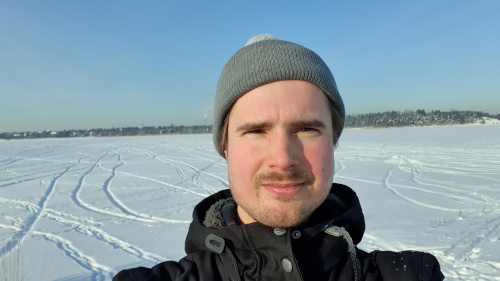
\includegraphics[width=\linewidth]{me1.jpg}
          \caption{Me in my beloved home town Helsinki in the middle of the summer (well, technically I am in Espoo, Otaniemi---and it is a snowy and shiny day in February, frozen sea seen in the background)}
        \end{figure}

        
        I am keeping up a blog that you can find in the blog posts section. It handles stuff encountered in my daily professional life. Stuff that I have found interesting. 
        

        \subsection{Education}
        \begin{itemize}
        \item 2025, PhD, \htmladdnormallink{``Narrow-Beam LEO and Stochastic Geometry Analysis: Non-Temporal and Temporal analysis,''}{dissertation.pdf} Department of Signal Processing, Aalto University\\
        \item 2018, Master of Philosophy, \htmladdnormallink{``Elementtimenetelmä (Finite Element Method),''}{https://helda.helsinki.fi/handle/10138/273474} Department of Applied Analysis, University of Helsinki, grade: 4/5
        \item 2016, Bachelor of Science, \htmladdnormallink{``Optimiohjausteoriasta ja sen sovelluksista (On Optimal Control Theory and Its Applications),''}{https://www.overleaf.com/project/563b9dec737da16f65bd24f2} University of Helsinki\\
          
        \end{itemize}

        
        
        \subsection{Publications}
        

        \begin{itemize}
        \item
          I. Angervuori and A. Afridi, ``Spatial and Temporal Correlation of the Interference in a Narrow-Beam LEO Network with ALOHA Medium Access Control,'' 2025, in IEEE Letters on Communications, submitted.
        \item
          I. Angervuori and R. Wichman, ``Order Statistics of the SIR and Interference Cancellation in a Narrow-Beam LEO Uplink,'' in IEEE Letters on Communications, 2025, submitted.
        \item
I. Angervuori, M. Haenggi and R. Wichman, ``Meta Distribution of the SIR in a Narrow-Beam LEO Uplink,'' in IEEE Transactions on Communications, 2025, doi: 10.1109/TCOMM.2025.3547734.
        \item
          I. Angervuori and R. Wichman, ``A Closed-Form Approximation of the SIR Distribution in a LEO Uplink Channel,'' 2022 IEEE Globecom Workshops (GC Wkshps), Rio de Janeiro, Brazil, 2022, pp. 856-861, doi: 10.1109/GCWkshps56602.2022.10008485.
        \item
          N. Okati, T. Riihonen, D. Korpi, I. Angervuori and R. Wichman, ``Downlink Coverage and Rate Analysis of Low Earth Orbit Satellite Constellations Using Stochastic Geometry,'' in IEEE Transactions on Communications, vol. 68, no. 8, pp. 5120-5134, Aug. 2020, doi: 10.1109/TCOMM.2020.2990993.
        \item A. Yastrebova et al., ``Theoretical and Simulation-based Analysis of Terrestrial Interference to LEO Satellite Uplinks,'' GLOBECOM 2020 - 2020 IEEE Global Communications Conference, Taipei, Taiwan, 2020, pp. 1-6, doi: 10.1109/GLOBECOM42002.2020.9347980.
        \item Niloofar Okati, Islam Tanash, Taneli Riihonen, Ilari Angervuori, Wichman Risto, ``Performance Evaluation of Low Earth Orbit Communication Satellites,'' Proceedings of XXXV Finnish URSI Convention on Radio Science, 2019
        \item Ilari Angervuori, Wichman Risto, Niloofar Okati, Taneli Riihonen, ``On routing protocols in inter-satellite communications,'' Proceedings of XXXV Finnish URSI Convention on Radio Science, 2019
          
        \end{itemize}

        \subsection{Personal grants}
        \begin{itemize}
          \item 2022, Väisälä Fund, funding for a research visit to the University of Notre Dame, 4349€
        \end{itemize}        
        \subsection{Thesis's and other projects}
        \begin{itemize}
        \item PhD dissertation: a sketch (not published) ``Narrow-Beam LEO and Stochastic Geometry Analysis: Non-Temporal and Temporal analysis,'' \htmladdnormallink{V.0.1}{dissertation.pdf}, Department of Electrical Engineering, Aalto University 2025          
        \item Master's thesis ``Elementtimenetelmä (The Finite Element Method),'' \htmladdnormallink{https://helda.helsinki.fi/handle/10138/273474}{https://helda.helsinki.fi/handle/10138/273474}, Department of Applied Analysis, University of Helsinki, 2018, grade: eximia cum laude (5/5)
        \item Bachelor's thesis ``Optimiohjausteoriasta ja sen sovelluksista (On Optimal Control Theory and Its Applications),'' \htmladdnormallink{https://www.overleaf.com/project/563b9dec737da16f65bd24f2}{https://www.overleaf.com/project/563b9dec737da16f65bd24f2}, University of Helsinki, 2016, grade: 4/5         
        \item An university project for a poster session, ``X-ray tomography with sparse data,'' \htmladdnormallink{https://www.dropbox.com/s/88pr2da24dil460/projektitosaulijamina.jpg?dl=0}{https://www.dropbox.com/s/88pr2da24dil460/projektitosaulijamina.jpg?dl=0}, 2015
          
        \end{itemize}
        
        \subsection{Other certificates}
        \begin{itemize}
        \item 2024, IEEE Transactions, Mobile Computing, \htmladdnormallink{2024 Review Certificate}{\reviewcert}
        \end{itemize}        
        

        \section{Blog posts 2021}
        Thinking thoughts.

        \subsection{January---Poisson process on a sphere}
        The \htmladdnormallink{Poisson point process}{https://en.wikipedia.org/wiki/Poisson_point_process} can be generalized to general \htmladdnormallink{manifolds}{https://en.wikipedia.org/wiki/Manifold}. In Particular, the Poisson process on a three-dimensional sphere surface is useful. Nicely enough, the Poisson process on a unit sphere is equivalent to the process in a two-dimensional area $ A = [-\pi,\pi] \times [-1,1]$ through the area-preserving mapping from $A$ to geographical coordinates
        \begin{equation}
          (x,y) \mapsto (1,x,\sin^{-1}(y)) \nonumber.
        \end{equation}


        The resulting process interpreted in geographical coordinates $(r,\theta,\varphi)$ is a Poisson point process on a sphere of radius $r$. The following code returns a scatter plot of Poisson points on the unit sphere.



        GNU Octave or Matlab:
\begin{verbatim}
%Plot random points on a unit sphere. Returns the points in a vector ref in cartesian coordinates
function refc = poissononsphere(density)
  yMin = -1; yMax = 1;
  xMin = -pi; xMax = pi;
  
  xDelta = xMax - xMin; yDelta = yMax - yMin; %Rectangle dimensions
  numbPoints = poissrnd(density);    %Number of points in the area is a Poisson variable of intensity given as density
  x = xDelta*(rand(numbPoints,1)) + xMin;    %Pick points from uniform distribution
  y = yDelta*(rand(numbPoints,1)) + yMin;    %Map referencepoints to geographical coordinates

  refs = [x'; asin(y)'];%Map geographical coordinates to Cartesian coordinates on a unit circle
  r = 1;
  refc = [r*sin(refs(2,:)+pi/2).*cos(refs(1,:)+pi);...
          r*sin(refs(2,:)+pi/2).*sin(refs(1,:)+pi);...
          r*cos(refs(2,:)+pi/2)];

  figure(1)    %Plot
  [X, Y, Z] = sphere;
  surf(X,Y,Z,'EdgeColor','none','FaceColor','black');
  hold on
  scatter3(refc(1,:),refc(2,:),refc(3,:),10,...
           'MarkerFaceColor','yellow',...
           'MarkerEdgeColor','red');
  axis equal
end
\end{verbatim}

Python:

\begin{verbatim}
import numpy as np
import scipy.stats
import matplotlib.pyplot as plt
from mpl_toolkits.mplot3d import axes3d

#Rectangle dimension
xMin = -np.pi; xMax = np.pi;
yMin = -1; yMax = 1;
xDelta = xMax - xMin; yDelta = yMax - yMin; #rectangle dimensions

#Density parameter of the Poisson point process. Mean number of points on the sphere
lambda0=1000; 

#Simulate Poisson point process

#Number of point in the area is a Poisson variable of intensity lambda0
numbPoints = scipy.stats.poisson( lambda0 ).rvs()
x = xDelta*scipy.stats.uniform.rvs(0,1,((numbPoints,1)))+xMin
y = yDelta*scipy.stats.uniform.rvs(0,1,((numbPoints,1)))+yMin

#Transform to geographical coordinates
x = x
y = np.arcsin(y)
#Plotting
fig = plt.figure()
ax = plt.axes(projection="3d")
ax.scatter(np.sin(y+np.pi/2)*np.cos(x+np.pi),np.sin(y+np.pi/2)*np.sin(x+np.pi),np.cos(y+np.pi/2), color='r' )
plt.show()

\end{verbatim}

Wolfram Language:
\begin{verbatim}
(*lambda is the mean number of points on the unit sphere*) 
  poissononsphere[lambda_] := 
  Module[{nrofpoints, phi, theta, radius, refc, polarp}, 
   nrofpoints = RandomVariate[PoissonDistribution[lambda]];
   polarp = 
    Table[{RandomVariate[UniformDistribution[{-Pi, Pi}]], 
      ArcSin[RandomVariate[UniformDistribution[{-1, 1}]]]}, 
     nrofpoints];
   radius = 1;
   refc = 
    Table[{radius*Sin[polarp[[i]][[2]] + Pi/2]*
       Cos[polarp[[i]][[1]] + Pi],
      radius*Sin[polarp[[i]][[2]] + Pi/2]*Sin[polarp[[i]][[1]] + Pi],
      radius*Cos[polarp[[i]][[2]] + Pi/2]}, {i, nrofpoints}];
   refc
   ];
   ListPointPlot3D[poissononsphere[500], BoxRatios -> {1, 1, 1}]  
\end{verbatim}

\begin{figure}
  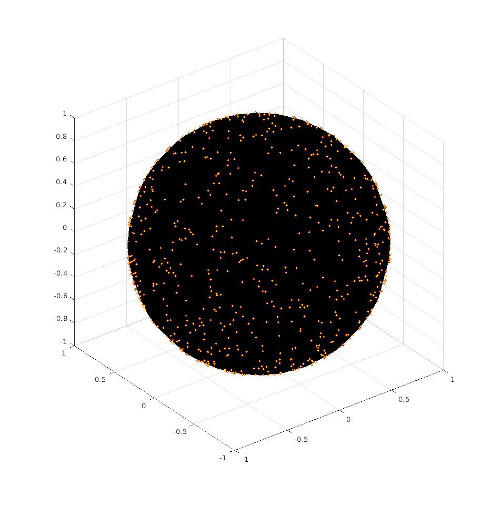
\includegraphics[width=\linewidth]{poissononsphere.jpg}
  \caption{Are the stars Poisson distributed in the sky?}
\end{figure}

\begin{figure}
  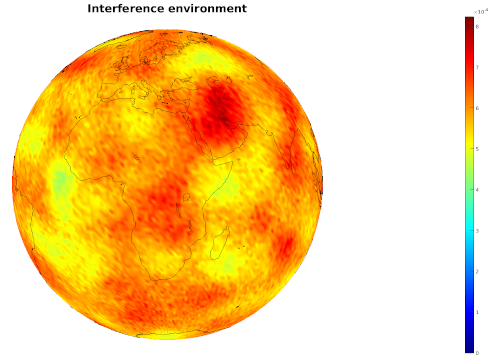
\includegraphics[width=\linewidth]{interferenceenvironment.png}
  \caption{Aggregate interference in a satellite. A color represents aggregate interference power at the given location. The interfering sources are considered Poisson distributed on Earth.}
\end{figure}

References:
\begin{itemize}
\item D. J. Daley and D. Vere-Jones, The General Poisson Process in  ``An introduction to the theory of point processes''. New York: Springer, 2003, pp. 39. 
\item Stoyan, Dietrich. et al. ``Stochastic Geometry and Its Applications''. 3rd ed. Chichester: Wiley, 2013. Print.
\item  \htmladdnormallink{H. Paul Keeler's Blog}{https://hpaulkeeler.com/simulating-a-poisson-point-process-on-a-sphere}
\end{itemize}




\subsection{February---Controlling your passwords with pass}
Pass is a nice Unix style free and open source wallet for keeping your passwords safe. Here is a brief look how to set it up in Linux.

\begin{itemize}
\item Install the application in the terminal. \\
\begin{verbatim}
sudo apt install pass  
\end{verbatim}
\item Check for the existing GPG keys. \\
\begin{verbatim}
gpg --list-keys 
\end{verbatim}
\item If no keys were found generate a key pair. \\
\begin{verbatim}
gpg --generate-key
\end{verbatim}
\item Copy the name of the key and initialize pass.\\
\begin{verbatim}
pass init ABCDEFGHIJKLMNOPQRSTUV1234
\end{verbatim}
where ABCDEFGHIJKLMNOPQRSTUV1234 is the name of the key.
\item Generate a password with \\
\begin{verbatim}
pass generate keyfolder/newkey 
\end{verbatim}
List the passwords.
\begin{verbatim}
pass
\end{verbatim}
Copy a password to the clipboard. \\
\begin{verbatim}
pass keyfolder/newkey -c
\end{verbatim}
For more commands:
\begin{verbatim}
man pass
\end{verbatim}
\end{itemize}

Connect Pass to Git and it is easy to keep track of passwords with multiple machines.
\begin{itemize}
\item Export your public and private key to a file with \\
\begin{verbatim}
  gpg --export --output public.key ABCDEFGHIJKLMNOPQRSTUV1234 
  gpg --export-secret-key --output private.key ABCDEFGHIJKLMNOPQRSTUV1234
\end{verbatim}
where ABCDEFGHIJKLMNOPQRSTUV1234 is your key name.\\
\item Now, we can initialize the Git repository with these keys. Move the public key and private key through a safe channel to a computer you wish to use Pass in. Import the keys to the machine: \\
\begin{verbatim}
gpg --import public.key
gpg --import private.key
\end{verbatim}
\item After importing the keys to a new machine you can list the keys:
\begin{verbatim}
gpg --list-keys 
\end{verbatim}
\item and initialize Pass with
\begin{verbatim}
pass init ABCDEFGHIJKLMNOPQRSTUV1234
\end{verbatim}
\item First, remember to \htmladdnormallink{add your public SSH key to GitHub}{https://docs.github.com/en/authentication/connecting-to-github-with-ssh/adding-a-new-ssh-key-to-your-github-account}. We will initialize the GitHub repository. If you do this for the first time, create a new repository named ``pass-store'' before the following commands. If the first command asks you to identify yourself, follow the instructions.
\begin{verbatim}
pass git init 
pass git remote add origin git@repo.com:myname/pass-store
\end{verbatim}
\item Get password data from the server (from a non-empty repository, otherwise skip)
\begin{verbatim}
pass git pull origin master --allow-unrelated-histories
pass git commit -am "firstcommit"
\end{verbatim}
If Git complains about ``divergent branches'' just choose the ``merge'' reconcileing and repeat the command.
\item Do some changes and pass will automatically commit them. Push and set the ``upstream''. \\
\begin{verbatim}
pass git push --set-upstream origin master 
\end{verbatim}
\item From here on you can use the familiar git commands. \\
\begin{verbatim}
pass git pull 
pass git push 
\end{verbatim}
It can be the case that you have to raise the trust level of the public key. For that, check \htmladdnormallink{this}{https://stackoverflow.com/questions/33361068/gnupg-there-is-no-assurance-this-key-belongs-to-the-named-user}  article. 
\end{itemize}
Stay safe :)


References:

\begin{itemize}
\item \htmladdnormallink{Password Store}{\pass}
\end{itemize}


\subsection{March---Signal propagation in a city}
Mobile telephone signal propagation in a city is characterized by obstacles, such as buildings and cars, that \htmladdnormallink{attenuate}{https://en.wikipedia.org/wiki/Attenuation}, \htmladdnormallink{reflect}{https://en.wikipedia.org/wiki/Reflection_(physics)}, \htmladdnormallink{refract}{https://en.wikipedia.org/wiki/Reflection_(physics)} and \htmladdnormallink{diffract}{https://en.wikipedia.org/wiki/Diffraction} the signal. Should there be a pure line-of-sight from the transmitter to the receiver, the receiver will always receive a constant power from the transmitter conditioned that the transmitter stays at a constant distance from the receiver---this can be the case, for example, if you are transmitting to a near-by high base-station antenna. Without the line-of-sight component, the signal strength will vary according to \htmladdnormallink{Rayleigh fading}{\ray} as the transmitter or the obstacles move. If only a limited line-of-sight element is present, the signal strength will follow \htmladdnormallink{Rician fading}{\ric} statistics.

I animated a couple of GIFs to help us perceive what is happening. The first figure demonstrates how a simple sine signal propagates between buildings. You can observe how the multi-path components sum up to a signal amplifying in some locations and degenerating in others. In the first figure, you can look for Rician conditions (lower right) and Rayleigh conditions (lower left) and see how the signal behaves. The figure was obtained by solving the Helmholtz equation by finite element method.

The second figure shows how the aggregate signal power from many mobile transmitters develops in time under Rician fading conditions. The aggregate power can be considered as interference in a receiver. You can see how the high peaks of interference power emerge at random locations. These kinds of peaks can cause decreased data rates. The figure was obtained by simulating a random walk of points in a realization of the Poisson point process on a plane.

\begin{figure}
  \includegraphics[width=\linewidth]{sin.gif}
  \caption{The white boxes represent buildings, and the little white circle is the transmitter. One can see how reflections will cause the aggregate signal strength to fluctuate by location depending on the phases of the incoming reflected waves.}
\end{figure}



\begin{figure}
  \includegraphics[width=\linewidth]{rician.gif}
  \caption{The interference power field develops in time as the interfering transmitters are moving in random directions at each time step. Red color represents the highest mean power of interference, and deep blue represents the absence of any interference. We assume  Rician fading. The interference in the red occurrences will reduce the performance remarkably.}
\end{figure}


References:
\begin{itemize}
\item François Baccelli, Bartlomiej Blaszczyszyn \htmladdnormallink{Stochastic Geometry and Wireless Networks, Volume I -Theory}{\hal}

\item Nicolae Cindea (2021).   \htmladdnormallink{Movie to GIF Converter}{https://www.mathworks.com/matlabcentral/fileexchange/17463-movie-to-gif-converter)}, MATLAB Central File Exchange. Retrieved June 14, 2021. 
\end{itemize}


%% \subsection{April – Frequentist inference in Mathematica}

%% Mathematica provides a package called “Hypothesis Testing” for analyzing random data. The package includes handy objects like “Around”, representing a quantity and the uncertainty around it. The following example code returns an Around object representing the confidence interval of the estimated bias of a coin after a repeated trial. As shown in the code, the ListPlot plots Around objects as such.

%% \begin{verbatim}
%% (*Load the Hypothesis Testing Package.*)
%% Needs["HypothesisTesting`"];

%% coin[flips_, bias_] :=
%%  (*Make the experiment and collect the data*) 
%%  Module[{index, realizations, mean, conf, around},
%%   realizations = {};
%%   For[index = 1, index <= flips, index++,
%%    realizations =  
%%      Append[realizations, 
%%       RandomVariate[BernoulliDistribution[bias]]];
%%    ];
  
%%   (*Mean*)
%%   mean = Mean[realizations[[All]]];
%%   (*Confidence interval*)
%%   conf = MeanCI[realizations[[All]]];
%%   (*Around object*)
%%   around = Around[mean, Abs[conf[[1]] - conf[[2]]]]
%%   ]
%% around = coin[1000, 0.5]
%% ListPlot[{around}]
%% \end{verbatim}

%% References:
%% \begin{itemize}
%% \item \htmladdnormallink{reference.wolfram.com}{https://reference.wolfram.com/language/guide/HypothesisTests.html}
  
%% \end{itemize}


\subsection{May---Rayleigh fading audiolized}

When a signal propagates through multiple paths, each signal component in each path will be in a different phase and of varying strength when received. Should there be no line-of-sight component present, the additive signal will fade according to the \htmladdnormallink{Rayleigh fading}{\ray}.

For example, a simple sine wave

\htmladdnormallink{wave}{https://soundcloud.com/ilari-angervuori/ref/s-MvjJzhr6qQH} (links to soundcloud.com---VOLUME ALERT)

can after some multi-path propagation sound like

\htmladdnormallink{this}{https://soundcloud.com/ilari-angervuori/ez-1/s-eQvc2PWfIJs}:

Assuming that the receiver is moving, the variation of Doppler shifts in different signal paths will cause the signal strength to vary randomly in time.

If we add some \htmladdnormallink{Gaussian white noise}{\gaus}, we notice that the original signal is somehow recognizable from the

\htmladdnormallink{noised signal}{https://soundcloud.com/ilari-angervuori/refnoise/s-Za1jUDgCPSV} (listen carefully, and you will hear the sine signal in the background).


but the

\htmladdnormallink{faded signal}{https://soundcloud.com/ilari-angervuori/eznoise/s-z4MjfqRZr6E}


will sometimes get buried under the noise---these events are referred to as \textit{deep fades}.


\begin{figure}
  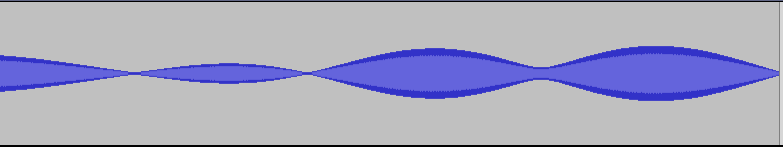
\includegraphics[width=\linewidth]{fadedsinesignal.png}
  \caption{The \htmladdnormallink{Envelope}{https://en.wikipedia.org/wiki/Envelope_(waves)} of a multi-path faded sine signal.}
\end{figure}

Here is a GNU Octave or Matlab code for the used Rayleigh simulator, which outputs the signal as audio:
\begin{verbatim}
%Rayleigh simulator. Jakes model. In Octave remember to load the statistics package.

close all
clear all

tic

N = 20; %Number multipaths.
T = linspace(0,10000,100000); %Time.
v = 0.001; %Speed of the receiver.
randan = pi*rand(1,N); %Random angles w.r.t. receiver.
rI = 1000*rand(1,N); %Random distances of the sources.

%Geometrical stuff. Check for the Jakes model in the reference.
An = @(t) (atan(sin(randan).*rI./(cos(randan).*rI-v*t))).*(cos(randan).*rI>v*t)+...
(pi-atan(sin(randan).*rI./(v*t-cos(randan).*rI))).*(cos(randan).*rI<=v*t);
phis = 2*pi.*(rand(1,N));
wc =pi/2; %Frequency of the signal.
Beta = 2*pi/(1/(wc/(2*pi)));
theta = @(t) cos(An(t)).*Beta*v.*t+phis;

powers = rand(1,N); %Random powers of the signals in the multipaths.
powers = powers./sum(powers); %Normalize the powers.
Ez = @(t) sum(powers.*cos(wc*t+theta(t)));
EZ = []; %Faded signal.
REF = []; %Original signal.
NOISE = []; %Additional Gaussian noise.
for t =T
EZ = [EZ Ez(t)];
REF = [REF cos(wc*t)];
NOISE = [NOISE 0.9*stdnormal_rnd(1)];
end

%Write the audio files at sampling rate 8000.
audiowrite('EZ.wav',EZ,8000)
audiowrite('EZNOISE.wav',1/2*(EZ+NOISE),8000)
audiowrite('REFNOISE.wav', 1/2*(REF+NOISE), 8000)


toc
plot(T,EZ)
\end{verbatim}


And the same in Python:

\begin{verbatim}
  import numpy as np
  import math
  import matplotlib.pyplot as plt
  import sounddevice as sd
  import time

  #Jakes Rayleigh simulator. Please check for the reference in this site for further details.

  N = 20 #Number of multipaths.
  T = np.linspace(0, 10000, 100000) #Time vector.
  v = 0.001 #Speed of the receiver. 



  randan = np.random.rand(1, N) * math.pi #Random angles w.r.t. receiver.
  rI = np.random.rand(1, N) * 1000 #Random distances of the sources.
  phis = np.random.rand(1, N) * 2 * math.pi 

  def An(t):
  return (np.arctan(np.sin(randan) * rI / (np.cos(randan) * rI - v * t))) * (
  np.cos(randan) * rI > v * t
  ) + (np.pi - np.arctan(np.sin(randan) * rI / (v * t - np.cos(randan) * rI))) * (
  np.cos(randan) * rI <= v * t
  )

  wc = np.pi/2 #Frequency of the signal.
  Beta = 2 * math.pi / (1 / (wc / (2 * math.pi)))

def theta(t):
    return np.cos(An(t)) * Beta * v * t +phis

powers = np.random.rand(1,N)*2 #Random powers of the signals in the multipaths.
powers = powers/np.sum(powers) #Normalize powers..

def Ez(t):
    return np.sum(powers * np.cos(wc * t + theta(t)))

EZ = np.vectorize(Ez)(T)
REF = np.vectorize(lambda time : 2*np.cos(wc * time))(T)

#Play and plot.
fs = 8000
sd.play(EZ,fs,blocking = True)
#sd.play(REF,fs,blocking = True)
plt.plot(T, EZ)
plt.show()  
\end{verbatim}



References:
\begin{itemize}
\item William C. Jakes, ``Microwave Mobile Communications'', IEEE PRESS, 1974.
\end{itemize}



\subsection{June---Why does MIMO work?}

Multiple-input and multiple-output \htmladdnormallink{MIMO}{https://en.wikipedia.org/wiki/MIMO} antenna technology is used to exploit the \htmladdnormallink{multi-path propagation}{\ray} to improve the capacity of a communication link. In principle, the link's capacity can be increased merely by increasing the power of the transmitting antenna. However---apart from being energy-consuming---this also increases interference to any other receivers should they operate in the same frequency band. In MIMO, the energy is divided among multiple antennas, and the link capacity is improved without using any extra energy and without increasing interference towards other transmitters.

Why does it work? Here is how I came up with a simple argument based on stochastic geometry. First, let us make some assumptions. We assume a flat and infinite Earth (this is a ``tin foil assumption,'' but it is often reasonable). In addition, our communication channel environment consists of many obstacles so that our transmitting and receiving antennae can not see each other. We are in a city full of houses, cars, trees, etc. Then, our data signal propagates to the receiver through multiple paths, for example, through distinct streets around different houses. The aggregate signal in the receiver will be  \htmladdnormallink{Rayleigh faded}{\ray}. The city is stormed with mobile phones exchanging data with their base stations, which further hand the data to the receiving mobile phones' base station and, on the other hand, cause interference to the other base stations. We assume that the interfering base stations are independently located and are distributed according to the \htmladdnormallink{Poisson point process}{https://en.wikipedia.org/wiki/Poisson_point_process}.

Let's consider that person A is sending a message to person B. We are interested in the probability that the base station serving person A successfully transmits the message to a base station serving person B. Under the assumptions above and some other simplified assumptions, as derived in \htmladdnormallink{here}{\hall}, we can express the probability of a successful transmission as:

\begin{equation}
  \textbf{P}[\text{Successful single-antenna transmission}] = e^{-\frac{\pi^2}{2\sqrt{P}}},
\end{equation}

where $P$ denotes the mean transmitting power of the base stations.

In MIMO, we use multiple distinct antennas to transmit the same message. In each antenna, the encoding of the message should be different so that it can't mix with the information that the other antennas are transmitting---this is possible by \htmladdnormallink{orthogonal modulation}{https://en.wikipedia.org/wiki/Orthogonal_frequency_division_multiplexing}.
Assuming that each message from each antenna independently propagates to the receiver, we can calculate from equation $(1)$ by the complementary probability that \textbf{at least one message transmission gets through:}

\begin{equation*}
  \textbf{P}[\text{Successful MIMO transmission with N antennas}]  = 1-\left(1-e^{-\frac{\pi^2}{2\sqrt{P/N}}}\right)^N,
\end{equation*}

where $N$ is the number of transmitting antennas. Notice that we divided the transmitting power $P$ by the number of antennas, so we didn't increase the aggregate power.
On the other hand, should we have no MIMO technology at hand, we could improve the link quality by increasing the power $P$ of a single antenna. In the following figure, we compare these two cases.

\begin{figure}
  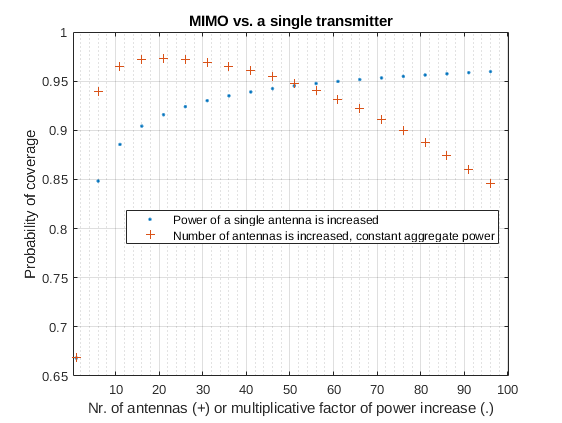
\includegraphics[width=\linewidth]{MIMO.png}
  \caption{MIMO saves energy and improves performance.}
\end{figure}

It is evident that MIMO is an excellent solution for increasing the throughput of a wireless communication link. Using multiple antennas, we can save power and achieve better data rates than by merely increasing the power of a single transmitter. In MIMO, using multiple antennas, statistically speaking, a significant fraction of the channels are in a good state (as well as a bad state), and the performance is consistent.

References:
\begin{itemize}
\item François Baccelli, Bartlomiej Blaszczyszyn \htmladdnormallink{Stochastic Geometry and Wireless Networks, Volume 2 - Applications}{\hall}
\end{itemize}

%% \subsection{July – Animating GIFs in GNU Octave}

%% Often it is nice to plot your results as an animation. The following code demonstrates the most effective way to write GIFs in Octave that I could find. Example code outputs an animation of a \htmladdnormallink{complex base-band signal symbol}{https://en.wikipedia.org/wiki/Quadrature_amplitude_modulation} in noise. Code uses the quiver plot, but any other plot should do equally well. Matlab compatibility is not guaranteed.

%% \begin{figure}
%%   \includegraphics[width=\linewidth]{gifu.gif}
%%   \caption{Animated GIF of a noisy QAM symbol}
%% \end{figure}


%% The point is to loop through all frames and save them to a file after each other with functions \textit{getframe} and \textit{imwrite}. 

%% \begin{verbatim}
%% function writeGIF()
%%   clear all;
%%   close all;
%%   clear imread;
%%   clear imwrite;
  
%%   N = 100; %%Number of frames.

%%   %%We use quiver plot as an example, but any other plot works equally.
%%   signal = 5 + 5*i; %%Baseband symbol.
%%   signal = signal + randn(1) + randn(1)*i ;   %%Add some Gaussian noise.
%%   quiver(0,0,real(signal), imag(signal))
%%   axis([[-10, 10],[-10, 10]])

%%   %%Write the first frame.
%%   frame = getframe(); %%Get the current frame.
%%   imwrite(frame.cdata,'gifu.gif','gif','writemode','overwrite',...
%%           'LoopCount',inf,'DelayTime',0.1, 'Compression' , 'lzw');  %%Write the frame to gifu.gif and use delay time 0.1 seconds.
  
%%   for iii = 1 : N
%%     iii
%%     %%Write GIF.
%%     signal = 5 + 5*i; %%Baseband symbol.
%%     signal = signal  + rand(1) + randn(1)*i ;   %%Add some Gaussian noise.
%%     quiver(0,0,real(signal), imag(signal))
%%     axis([[-10, 10],[-10, 10]])
    
%%     frame = getframe(); %%Get the current frame.
%%     imwrite(frame.cdata, 'gifu.gif','gif','writemode','append','DelayTime',0.1, 'Compression' , 'lzw'); %%Write the frame to gifu.gif.
%%   end
%% end
%% \end{verbatim}
%% The 'Compression' setting is important to avoid insane file sizes and memory usage.

%% References: 
%% \begin{itemize}
%% \item \htmladdnormallink{Octave Image Processing}{https://octave.org/doc/v4.0.1/Loading-and-Saving-Images.html}
%% \end{itemize}


\subsection{August---Radio waves in a tunnel}

Almost everyone has some experience of how radio turns static when driving into a tunnel. The radio stations only work if a special  \htmladdnormallink{radiating cable}{https://en.wikipedia.org/wiki/Leaky_feeder} is installed inside the tunnel. Once upon a night, I could not sleep, pondering why the \htmladdnormallink{FM}{https://en.wikipedia.org/wiki/FM_broadcast_band} radios are unsuable in the tunnels. From my experience, mobile phone signals that operate at higher frequencies work better. Someone might have told me that FM radio wavelength is so large that the wave ``does not fit the tunnel''. But as intuitively acceptable as this explanation could be (I don't think it is even that), this answer did not satisfy me.


After some research, I found that the explanation lies in \htmladdnormallink{Maxwell equation's}{https://en.wikipedia.org/wiki/Maxwell's_equations} behavior (well, what a surprise). Everything backs down to the boundary conditions of the electromagnetic field at the tunnel wall: the tangential component of the electric field component of the electromagnetic wave has to be near zero in the tunnel interface---this leads to a situation where the wave has, in a sense, no room to oscillate inside the tunnel.


Intuitive or not, this is what the equations tell us. To demonstrate this, I solved using \htmladdnormallink{FEM}{https://en.wikipedia.org/wiki/Finite_element_method}, the \htmladdnormallink{Helmholtz equation}{https://en.wikipedia.org/wiki/Helmholtz_equation} for a plane wave in a two-dimensional setting mimicking a tunnel and its entrance. The \htmladdnormallink{electromagnetic wave's}{https://en.wikipedia.org/wiki/Electromagnetic_radiation} polarization is so that the electrical component is pointing at the right angle w.r.t. the plane (either towards or against the reader of this page). \htmladdnormallink{Boundary conditions}{https://en.wikipedia.org/wiki/Boundary_value_problem} inside the 2D tunnel is zero. The coloring represents the electrical component's magnitude.

We compare the behavior of two different wavelengths:




\begin{figure}
  \includegraphics[width=\linewidth]{highfreq.gif}
  \caption{High frequencies fit in the tunnel.}
\end{figure}


\begin{figure}
  \includegraphics[width=\linewidth]{lowfreq.gif}
  \caption{Wavelengths bigger than the diameter of the tunnel will not get through.}
\end{figure}.



References: 
\begin{itemize}
\item \htmladdnormallink{Scattering Problem: Matlab PDE Modeler App}{https://se.mathworks.com/help/pde/ug/scattering-problem.html}
\item \htmladdnormallink{Interface conditions for electromagnetic fields (Wikipedia article)}{https://en.wikipedia.org/wiki/Interface_conditions_for_electromagnetic_fields}
\end{itemize}

%% \subsection{September – The universality of the Poisson point process (breaking a pile of sand)}

%% The two-dimensional \htmladdnormallink{Poisson point process}{https://en.wikipedia.org/wiki/Poisson_point_process} appears everywhere in nature: locations of cell phones in a city, raindrops in a puddle,  locations of a bunch of grains of sand thrown in the ground, \textit{etc}.

%% As a fun example, let us study how a bunch of grains of sand arranged into a sand castle will spread by wind and water around the sunny beach and, finally, into a realization of the Poisson point process.

%% For simplicity, the sand castle is so tiny that it can be considered entirely located at the \htmladdnormallink{origin}{https://en.wikipedia.org/wiki/Origin_(mathematics)} of the two-dimensional beach. Let's assume that the amount of grains in the pile is  \htmladdnormallink{Poisson distributed}{https://en.wikipedia.org/wiki/Poisson_distribution}: In our model, the sand castle is a Poisson distributed random amount of sand piled above each other in the origin. We assume that the expected number of sand is $N$. Suppose that wind moves individual sand grains from the pile after a while, directing them with a uniformly distributed angle and to a random, normal distributed distance between $[0, \infty)$. In other words, the probability density function of the distance $|Y_i|$ of the sand grain $i$ is $y \mapsto  e^{-y^2/2}\sqrt{\frac{2}{{\pi}}} dy.$ 
  
%%   After a random translation of all points, the \htmladdnormallink{Laplace functional}{https://en.wikipedia.org/wiki/Laplace_functional} $ \mathcal{L}(f) \triangleq \mathbb{E}\exp \{-\sum f(x)\} $ of the \textit{distances} $\{|Y_i|\}_i$ is 

%%   \begin{align*}
%%     \mathcal{L}_{Y}(f) &= \mathbb{E}_{n,Y} \exp \left[-\sum_{i=1}^n f(|Y_i|) \right] = \mathbb{E}_{n}   \mathbb{E}_{Y} \prod_{i=1}^n\exp  \left[  -f(|Y_i|)   \right]  \\
%%     &= \mathbb{E}_{n}  \left[ \int_0^{\infty} \dots \int_0^{\infty}   \prod_{i = 1}^n\exp \left[  -f(y_i)  \right] \sqrt{\frac{2}{\pi}}e^{-y_i^2/2} dy_1 \dots d y_n \right] \\
%%     &= \mathbb{E}_n \left[  \left( \int_{0}^{\infty}  \exp \left[  -f(y)   \right] e^{-y^2/2}\sqrt{\frac{2}{\pi}}dy \right)^n\right] \\
%%     &=
%%     &= \mathbb{E}_n \exp \left[ \sum_{i=1}^n \log \left(   \int_{0}^{\infty}  \exp \left[  -f(y)  \right] e^{-y^2/2} \sqrt{\frac{2}{ \pi}} dy \right) \right]. (1) \\ 
%%   \end{align*}

%%   Next, we want to show that (1) have to form of the  \htmladdnormallink{Laplace functional}{https://en.wikipedia.org/wiki/Poisson_point_process\#Laplace_functionals} of the Poisson point process. Let  $\Phi \subset (0,\infty)$ be the Poisson process of density $\lambda$. We evaluate the Laplace tranform of $\Phi$ with $g(y) = - \log \left(\int_{0}^{\infty}  \exp \left[  -f(y)  \right] e^{-y^2} \sqrt{\frac{2}{ \pi}}dy \right)$:
%%   \begin{align*}
%%     \mathcal{L}_{Y}(f) =\mathcal{L}_{\Phi}(g) &= \exp \left[  -\int_{0}^{\infty} 1 -  e^{\log \left(   \int_{0}^{\infty}  \exp \left[  -f(y)   \right] \sqrt{\frac{2}{\pi}}e^{-y^2/2} dy \right) } \lambda dx \right]    \\
%%     &= \exp \left[-\int_{0}^{\infty} \left(1  -   \int_{0}^{\infty}  \exp [-f(y)] \sqrt{\frac{2}{\pi}}e^{-y^2/2}  dy \right)  \lambda dx  \right] \\
%%     &= \exp \left[-\int_{0}^{\infty}\lambda dx\int_{0}^{\infty} \left(1  -     \exp [-f(y)]   \right) \sqrt{\frac{2}{\pi}}e^{-y^2/2} dy    \right] \\ 
%%     &= \exp \left[-\int_{0}^{\infty} \left(1  -     \exp [-f(y)]   \right)  \sqrt{\frac{2}{\pi}}e^{-y^2/2}  N dy    \right], (2) \\   
%%   \end{align*}

%%   where $N$ denotes the expected number of points in the sand pile (\htmladdnormallink{Campbell's theorem}{https://en.Wikipedia.org/wiki/Campbell\%27s_theorem_(probability)}). The formula $(1)$ is the Laplace functional of the Poisson p.p. on $[0, \infty)$ with a density parameter $\sqrt{\frac{2}{\pi}}e^{-x^2} N$. As the direction of the translation of a sand grain was uniformly distributed, we can conclude that the sand grains are Poisson distributed according to the Poisson p.p. with the two-dimensional multivariate Gaussian distribution as the density. This construction may be an example of the universality of the Poisson point process in nature.
  
    
%%     \begin{figure}
%%       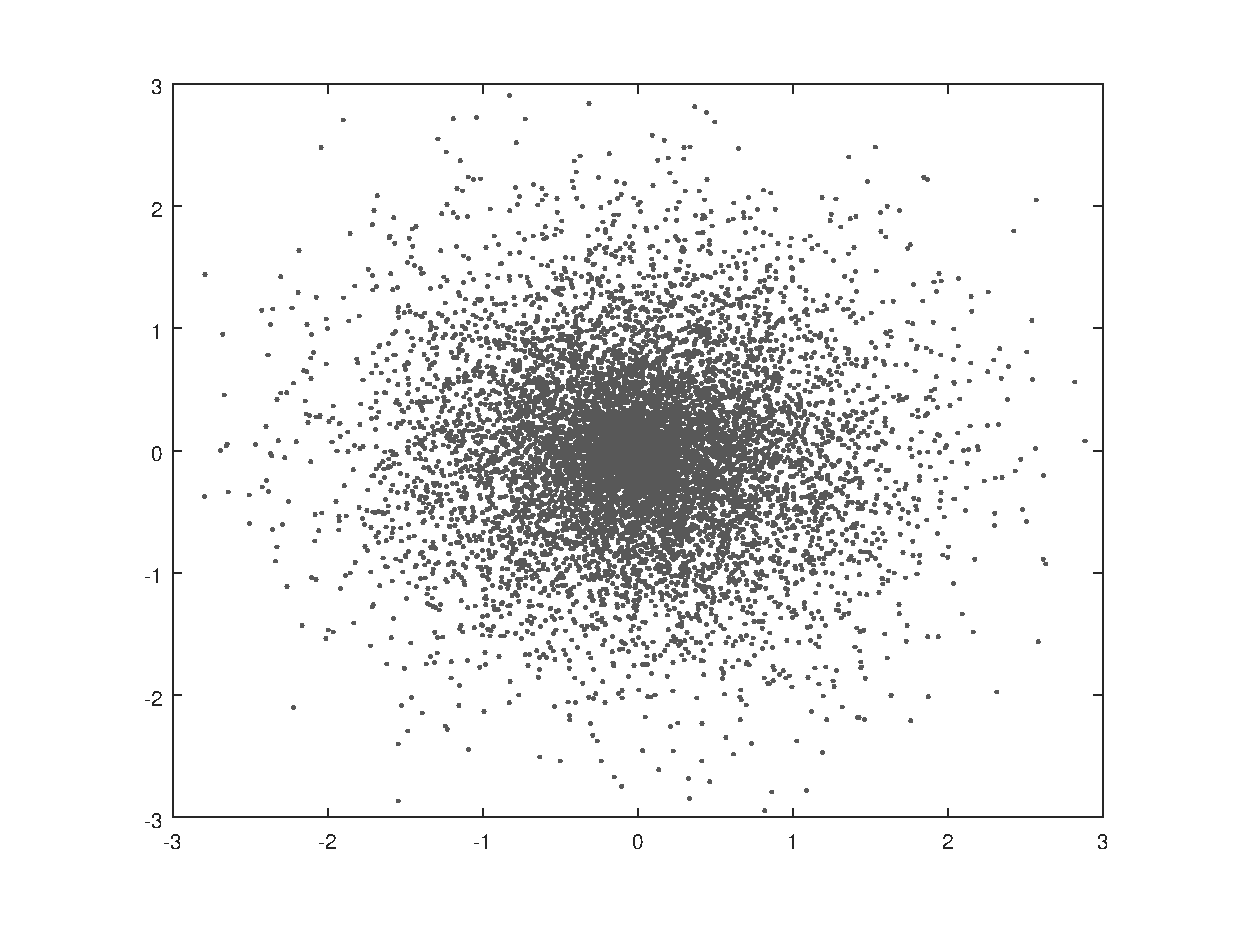
\includegraphics[width=\linewidth]{spread.eps}
%%       \caption{$10000$ points randomly moved from the origo to the plane.}
%%     \end{figure}.


%%     References:
%%     \begin{itemize}
%%     \item D. J. Daley and D. Vere-Jones, The General Poisson Process in  ``An introduction to the theory of point processes''. New York: Springer, Volume II: General Theory and Structure, 2008, pp. 166.   
%%     \item François Baccelli, Bartlomiej Blaszczyszyn \htmladdnormallink{Stochastic Geometry and Wireless Networks, Volume I -Theory}{\hal}
%%     \end{itemize}



    \subsection{October – Fast Fourier transform in GNU Octave}

    \htmladdnormallink{Fast fourier transform}{https://en.wikipedia.org/wiki/Fast_Fourier_transform} (FFT) is an algorithm that computes the \htmladdnormallink{discrete Fourier transform}{https://en.wikipedia.org/wiki/Discrete_Fourier_transform}.

    FFT is especially handy in real-time digital signal processing. Digital computers are working on discrete data, thus a input signal is always sampled with some sampling rate $F_s$ (Hz). By the \htmladdnormallink{Nyquist-Shannon sampling theorem}{https://en.wikipedia.org/wiki/Nyquist\%E2\%80\%93Shannon_sampling_theorem}, sampling captures frequencies under $F_s/2$.

    Octave calculates the FFT of a discrete signal.  In the following code, we calculate the normalized FFT and plot the frequency spectrum w.r.t. the frequency. Signal vector and sampling frequency are given as input.

\begin{verbatim}
##Calculates the FFT and plots the frequency spectrum of a signal. Sampletimes have to start at time 0.

function fftvector = plotfft(signal, Fs)
  N = length(signal); #Signal length.
  FFT =  fft(signal);
  if(mod(N,2) == 0) #Check if signal length is odd or even.
    FFT = 2*FFT(1 : N/2)/N;
    f = Fs*(0 : (N - 1)/2)/(N - 1); 
  else
    FFT = 2*FFT(1 : (N - 1)/2)/N;
    f = Fs*(0 : (N - 2)/2)/(N - 1);
  end  
  fftvector = [f; FFT];
  
  figure(1)
  plot(f, abs(FFT));
  title('Fast fourier transform')
  xlabel('Frequency (Hz)')
  print  plot.jpg
end

\end{verbatim}

The following figure shows my track \htmladdnormallink{Tappimarssi}{https://soundcloud.com/ilari-angervuori/tappimarssi} in the frequency domain. The track was imported to Octave by

\begin{verbatim}
[signal, Fs] = audioread('Tappimarssi.wav');
\end{verbatim}



\begin{figure}
  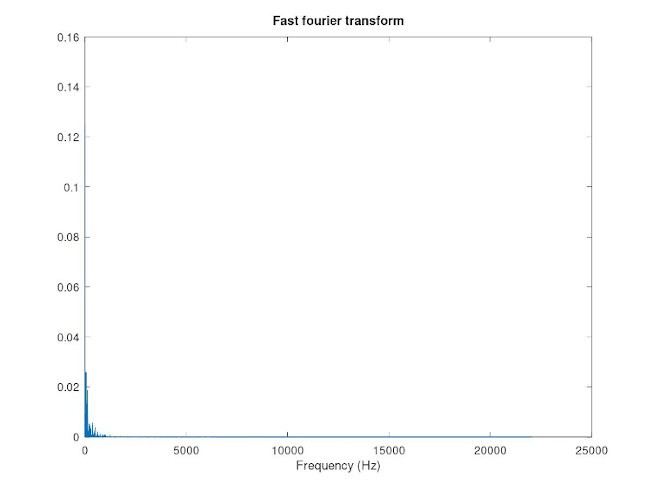
\includegraphics[width=\linewidth]{tappimarssi.jpg}
\end{figure}


\begin{itemize}
\item  \htmladdnormallink{Octave Documentation – Signal Processing}{https://octave.org/doc/v5.2.0/Signal-Processing.html}
\end{itemize}

\subsection{November – Digital filtering}

Let's construct a simple digital band-pass filter based in the \htmladdnormallink{sinc filter}{https://en.wikipedia.org/wiki/Sinc_filter}.

As everyone know, the sinc function is the \htmladdnormallink{impulse response}{https://en.wikipedia.org/wiki/Impulse_response} of a low-pass filter. That is, the \htmladdnormallink{convolution}{https://en.wikipedia.org/wiki/Convolution} of a signal $ S(t)$ and the sinc function $ t \mapsto \frac{\sin(2 \pi B_L t)}{\pi t}$ will produce a low-pass filtered signal $S(t)$ without frequencies higher than $B_L$. Similarly, the function $ t \mapsto \delta(t) -  \frac{\sin(2 \pi B_H t)}{\pi t},$ where $ \delta(t)$ represents the \htmladdnormallink{Dirac delta function}{https://en.wikipedia.org/wiki/Dirac_delta_function}, is the frequency response of the ideal high-pass filter of frequency $B_H$.

Heuristically, we can right away derive the discrete versions of the impulse responses:

$$
\mathbb{Z} \ni i \mapsto \frac{\sin(2 \pi \frac{B_L}{f_c} i)}{\pi i},
$$
for the low-pass filter, and

$$
i \mapsto \delta[i] - \frac{\sin(2 \pi \frac{B_H}{f_c} i)}{\pi i},
$$

for the high-pass filter. The variable $f_c$ is the sampling frequency and  $i \mapsto \delta[i] := \delta_{0i} $ is the \htmladdnormallink{Kronecker delta}{https://en.wikipedia.org/wiki/Kronecker_delta}.

Now, having a discrete signal at hand, band-pass filtering  is (in the simplest approach) just a matter of discrete convolution of the signal with the functions above. The following Octave code does the job.


\begin{verbatim}
##Sinc band-pass filter. f0 = B_L/fs, f1 = B_H/fs

function filtered = sincfilter(signal, f0, f1)
  if(mod(length(signal), 2) != 0) #Check if the signal length is even or odd.
    signal = signal(1 : length(signal) - 1);
  end
  
  M = 10000; #Increase this to increase accuracy.
  sincF = zeros(1, M);
  for m =  -M/2 + 1 : 1 : M/2 
    if(!(m  == 0))
      sincF(m + M/2) = sin(2*pi*f1*m)./(pi*m);
    else
      sincF(m + M/2) = 2*f1;
    end
  end

  sincH = zeros(1,M);
  for m =  -M/2 + 1 : 1 : M/2 
    if(!(m  == 0))
      sincH(m + M/2) = -sin(2*pi*f0*m)./(pi*m);
    else
      sincH(m + M/2) = -2*f0 + 1;
    end
  end
  
  ##Plot stuff.
  figure(1)
  plot(sincF)
  figure(2)
  plot(signal)

  tic
  filtered = conv(signal, sincF, "same");
  filtered = conv(filtered, sincH, "same");
  toc

  figure(3)
  plot(filtered)
end


\end{verbatim}



\begin{figure}
  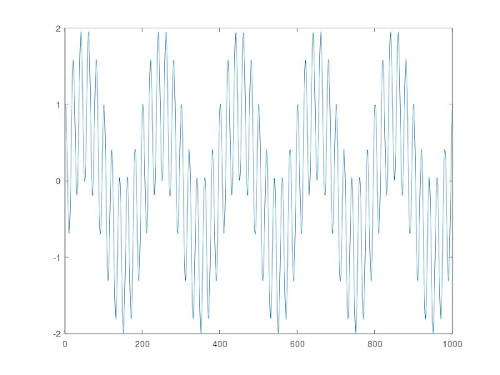
\includegraphics[width=\linewidth]{signal.jpg}
  \caption{Signal of form $\cos(20 \pi t) + \sin(2 \pi t)$}
\end{figure}

\begin{figure}
  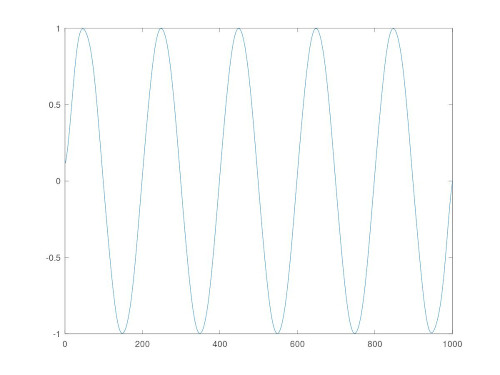
\includegraphics[width=\linewidth]{filtered.jpg}
  \caption{The same signal with the first term filtered away}
\end{figure}





For more accuracy and effectiveness, one should use windowed or recursive filters. One can check in the references for more sophisticated methods!


References:
\begin{itemize}
\item Steven W. Smith, ``Digital Signal Processing – A Practical Guide for Engineers and Scientists'', Elsevier Science, 2003.
\end{itemize}


%% \subsection{December – Contour plot in Mathematica}

%% A contour plot is a nice way to represent 2D data. Mathematica has some great tools for constructing such plots, but you might want to tweak the fonts and graphics a bit. Sometimes fonts should be enlarged so that they are visible e.g. in a journal article where there is not too much space to use.

%% The following code returns a contour plot of the \htmladdnormallink{Riemann zeta function's}{https://en.wikipedia.org/wiki/Riemann_zeta_function} absolute value in an area in the complex plane; $(-2,10) \times(-10i, 10i) \subset \mathbb{C}.$ Text fonts are enlarged from default. Only values under $\max = 2$ are plotted. Values above that are ``clipped'' away as white colour. By definition of the absolute value, values are always more than $0$, otherwise values under $0$ would get clipped away with black colour. Contours are drawn in intervals of $0.1$, as adjusted in the \textbb{Range} function.
%% \begin{verbatim}
%% max = 2;
%% ContourPlot[Abs[N[Zeta[x + y*I]]], {x, -2, 10}, {y, -10, 10}, 
%%  PlotLegends -> BarLegend[{"Rainbow", {0, max}}], 
%%  ColorFunction -> "Rainbow", ContourStyle -> Black, 
%%  Contours -> Function[{min, max}, Range[min, max, 0.1]], 
%%  PlotLabel -> 
%%   Style["Absolute value of the Riemann zeta function", 16, Bold], 
%%  BaseStyle -> {FontSize -> 15}, 
%%  FrameLabel -> {Style["Real axis" , 16, Bold], 
%%    Style["Imaginary axis", 16, Bold]}, PlotRange -> {0, max}, 
%%  ClippingStyle -> {Black, White}]
%% \end{verbatim}


%% \begin{figure}
%%   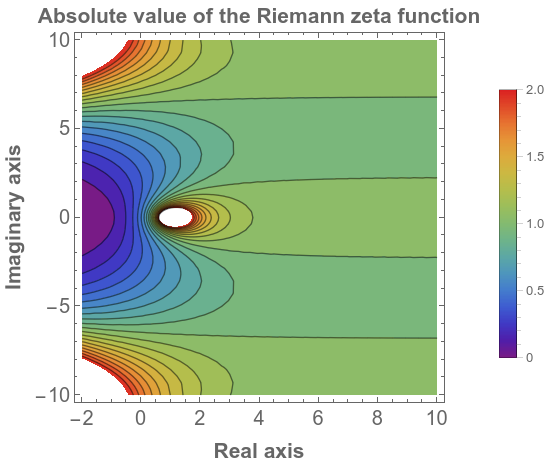
\includegraphics[width=\linewidth]{zeta.png}
%% \end{figure}



%% References:
%% \begin{itemize}
%% \item \htmladdnormallink{reference.wolfram.com}{https://reference.wolfram.com/language/guide/HypothesisTests.html}
%% \item Díaz-Francés, Eloísa; Rubio, Francisco J. (2012-01-24). "On the existence of a normal approximation to the distribution of the ratio of two independent normal random variables". Statistical Papers. Springer Science and Business Media LLC.
%% \end{itemize}


 \section{Blog posts 2022}
%%         General thoughts on mathematics and engineering, practical instructions, semi-artistic logical  nonsense. The themes of this blog are much inspired by the challenges encountered in my professional life. 

\subsection{January---Inverse of a Gaussian variable}

There is a lot of literature on the \htmladdnormallink{inverse}{https://en.wikipedia.org/wiki/Inverse_distribution} of a Gaussian distributed variable (this should not be fixed with inverse Gaussian distribution---it is a different matter). The inverse distribution is ill-behaved; the mean and variance do not generally exist.

I came up with a simple approximation that works well if the mean is large enough and the variance is small enough (I have yet to work out the details of the exact conditions for this approximation. However, the results can be verified, e.g., by Monte Carlo simulations).

First, approximate the Gaussian distributed variable $X \sim \mathcal{N}(\mu, \sigma^2)$ by a log-normally distributed variable $X \approx Y \sim \text{Lognormal}(\mu_{\text{LN}}, \sigma_{\text{LN}}),$ with corresponding mean and variance, \textit{i.e.}, $$\mu = \exp\left( \mu_{\text{LN}} + \frac{\sigma_{\text{LN}}^2}{2} \right)$$ and
$$\sigma = (\exp( \sigma_{\text{LN}}^2) - 1)\exp(2 \mu_{\text{LN}} + \sigma_{\text{LN}}^2).$$ We leave the solving of $\mu_{\text{LN}}$ and $\sigma_{\text{LN}}$ as an easy exercise for the reader. (:


Using the theory of log-normal distribution, the inverse of $X$ is now given by
$$
1/X \approx 1/Y \sim \text{Lognormal}(-\mu_{\text{LN}}, \sigma_{\text{LN}}).
$$

That's it!



References:
\begin{itemize}
\item \htmladdnormallink{Log-normal distribution}{https://en.wikipedia.org/wiki/Log-normal_distribution}
\item  Díaz-Francés, Eloísa; Rubio, Francisco J. (2012-01-24). "On the existence of a normal approximation to the distribution of the ratio of two independent normal random variables". Statistical Papers. Springer Science and Business Media LLC.
\end{itemize}


\subsection{February---Voronoi tesselation on a sphere}

Voronoi tessellation consists of neighborhood areas of a given set of points, or Voronoi cells: every cell is surrounded by the area that consists of locations that are closer to the cell than any other cell. The \htmladdnormallink{Voronoi Diagram}{https://en.wikipedia.org/wiki/Voronoi_diagram}, or Voronoi tessellation, has applications, \textit{e.g.}, in wireless communications. 

\begin{figure}
  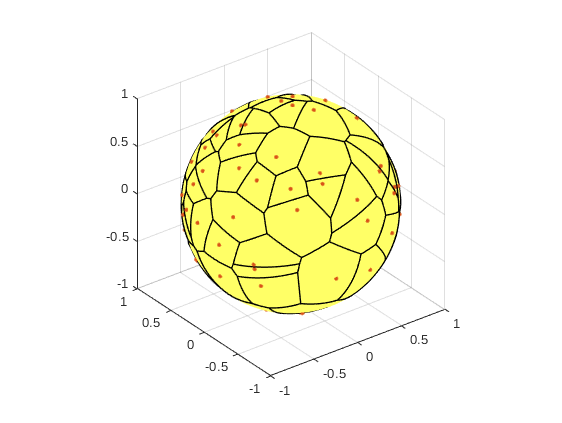
\includegraphics[width=\linewidth]{voronoionsphere.png}
\end{figure}


The next Matlab code produces a Voronoi tessellation on a sphere Poisson points as cells. It is based in Grady Wrights codes openly available in Github. 

\begin{verbatim}


%%Create Voronoi tesselation around Poisson points on a Sphere.

clear all;
close all;

addpath(fullfile(cd,'rbfsphere'));
density = 100;
X = poissononsphere(density)'; %Poisson points in spherical coordinates.
voronoiSph(X); %This function is downloaded from gradywright's Github. It is placed in the folder 'rbfsphere'.

function refc = poissononsphere(density)
  yMin = -1; yMax = 1;
  xMin = -pi; xMax = pi;
  
  xDelta = xMax - xMin; yDelta = yMax - yMin; %Rectangle dimensions
  numbPoints = poissrnd(density);    %Number of points in the area is a Poisson variable of intensity given as density
  x = xDelta*(rand(numbPoints,1)) + xMin;    %Pick points from uniform distribution
  y = yDelta*(rand(numbPoints,1)) + yMin;    %Map referencepoints to geographical coordinates
  ref = [x y]';

  refs = [x'; asin(y)'];%Map geographical coordinates to Cartesian coordinates on a unit circle
  r = 1;
  refc = [r*sin(refs(2,:)+pi/2).*cos(refs(1,:)+pi);...
          r*sin(refs(2,:)+pi/2).*sin(refs(1,:)+pi);...
          r*cos(refs(2,:)+pi/2)];
end

\end{verbatim}



References:
\begin{itemize}
\item \htmladdnormallink{gradywright Github}{https://github.com/gradywright/spherepts/tree/master/code}
\end{itemize}



%% \subsection{March – Plotting in Mathematica}

%% Here's a plot for Mathematica that you can use as a template to plot ListLinePlot and Plot in the same figure. Font sizes are increased to be well visible in a research article. 


%% \begin{verbatim}
%% xmax = 150;
%% ymax = 0.025;
%% Show[
 
%%  ListLinePlot[{Table[{t, 
%%      PDF[GammaDistribution[3.715287738432738`, 16.575007504627795`]][
%%       t]}, {t, 0, xmax, xmax/10}],
%%    Table[{t, 
%%      PDF[GammaDistribution[6.502676225156808`, 8.60919186301341`]][
%%       t]}, {t, 0, xmax, xmax/10}], 
%%    Table[{t, 
%%      PDF[GammaDistribution[3.3444580518527207`, 16.73897127052263`]][
%%       t]}, {t, 0, xmax, xmax/10}]}, 
%%   PlotRange -> {{0, xmax}, {0, ymax}},
%%   PlotLabel -> PDF,
%%   AxesLabel -> {Style["SIR", 16, Bold], Style["", 16, Bold]}, 
%%   PlotLegends -> Placed[{"Sim 1", "Sim 2", "Sim 3"}, Right], 
%%   PlotMarkers -> {Automatic, 10}, BaseStyle -> {FontSize -> 15}],
%%  Plot[
%%   {
%%    PDF[GammaDistribution[3.715287738432738`, 16.575007504627795`]][
%%     t],
%%    PDF[GammaDistribution[6.502676225156808`, 8.60919186301341`]][t],
%%    PDF[GammaDistribution[3.3444580518527207`, 16.73897127052263`]][t]
%%    }, {t, 0.01, xmax}, PlotStyle -> Thick, 
%%   PlotLegends -> 
%%    Placed[{"\[CapitalGamma](3.7, 16.6)", "\[CapitalGamma](6.5, 8.6)", 
%%      "\[CapitalGamma](3.3, 16.7)"}, Right]]
%%  ]
%% \end{verbatim}


%% Output:
%% \begin{figure}
%%   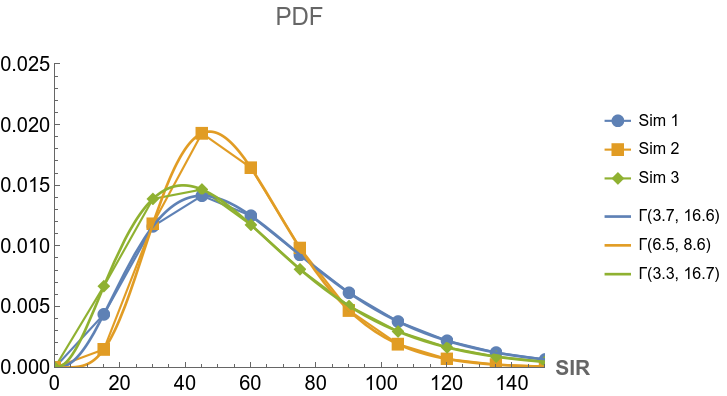
\includegraphics[width=\linewidth]{listlineplot.png}
%% \end{figure}


%% References:
%% \begin{itemize}
%% \item \htmladdnormallink{reference.wolfram.com}{https://reference.wolfram.com/language/ref/Plot.html}
%% \end{itemize}


%% \subsection{April – Satellite communication toolbox in Matlab}

%% Matlab's Satellite Communication Toolbox can be used to study and visualize satellite networks. The following code places a terrestrial station in Otaniemi, and a LEO satellite in $2000$ km tracking the station. Satellite have to be at least in a elevation angle of $35$ degrees to contact to the base station. Satellites field of view and a $3$ dB footprint of width $1.5$ degrees is also represented.

%% \begin{verbatim}
%% clear all;
%% close all;

%% startTime = datetime(2020,8,19,20,55,0); % 19 August 2020 8:55 PM UTC
%% stopTime = startTime + days(1);          % 20 August 2020 8:55 PM UTC
%% sampleTime = 60;                         % seconds
%% sc = satelliteScenario(startTime,stopTime,sampleTime);


%% semiMajorAxis = (6378 + 2000)*1000;          % meters
%% eccentricity = 0;
%% inclination = 90;                   % degrees
%% rightAscensionOfAscendingNode = 0; % degrees
%% argumentOfPeriapsis = 0;           % degrees
%% trueAnomaly = 0;                   % degrees
%% sat1 = satellite(sc, ...
%%     semiMajorAxis, ...
%%     eccentricity, ...
%%     inclination, ...
%%     rightAscensionOfAscendingNode, ...
%%     argumentOfPeriapsis, ...
%%     trueAnomaly, ...
%%                  "Name","Satellite", ...
%%                  "OrbitPropagator","two-body-keplerian");

%% sat1.LabelFontSize = 30;
%% cam1 = conicalSensor(sat1,"MaxViewAngle",90)
%% cam2 = conicalSensor(sat1,"MaxViewAngle",1.5/2)

%% name = "Test Transmitter";
%% minElevationAngle = 35; % degrees
%% lat = 60.185;
%% lon = 24.83;
%% geoSite = groundStation(sc, lat, lon, "Name", name, "MinElevationAngle", minElevationAngle)
%% geoSite.LabelFontSize = 30;
%% ac1 = access(cam1,geoSite);
%% ac2 = access(cam2,geoSite);

%% fov1 = fieldOfView(cam1, "LineColor",'blue', "LineWidth", 10)
%% ac1.LineColor = 'black';

%% fov2 = fieldOfView(cam2, "LineColor", 'green', "LineWidth", 10)

%% pointAt(sat1,geoSite);

%% play(sc);

%% \end{verbatim}



%% Output:
%% \begin{figure}
%%   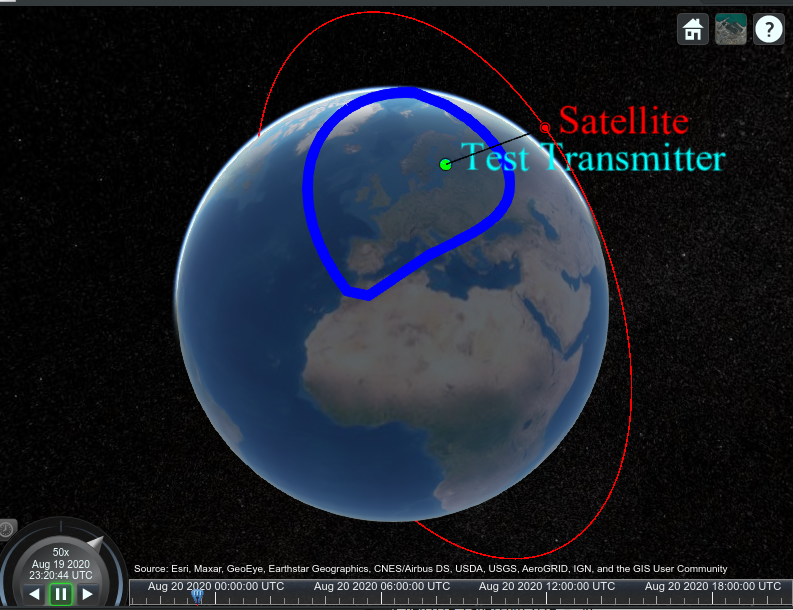
\includegraphics[width=\linewidth]{stk.png}
%% \end{figure}


%% References:
%% \begin{itemize}
%% \item \htmladdnormallink{Mathworks}{https://se.mathworks.com/products/satellite-communications.html}
%% \end{itemize}

\subsection{May – Digital to analog modulation}
Digital signal consists of values at discrete times, whereas analog signal is continuous in time $t$. As the orthogonal set of \htmladdnormallink{sinc functions}{https://en.wikipedia.org/wiki/Sinc_function}
$$
\{t \mapsto \text{sinc}(F_s t - n)\}_n,
$$
spans the space of signals of bandwidth $F_s/2$, an analog signal can be (uniquely) produced from a digital signal of length $N$ 
$$
\{ x[n]\}_{n=0}^{N-1}
$$
as a superposition of the \text{sinc} basis-functions
$$
S(t) =\sum_{n = 0}^{N-1} x[n]\text{sinc}(F_s t - n),
$$
where $F_s$ is the sampling rate of the digital signal.

The following GNU Octave function produces the analog signal from a given digital signal

\begin{verbatim}
%%Function returns the values at times T of the analog signal of the corresponding digital signal sampled at speed Fs.
function xb = digitaltoanalog(T, digitalsignal, Fs)
  xb = [];
  for t = T
    xb =  [xb sum(digitalsignal.*sinc(Fs*t - (0 : length(digitalsignal) - 1)))];
  end
end
\end{verbatim}

The following code simulates a rectangle pulse train signal given as input, samples the input to a digital signal $x$, and modulates the sampled digital signal back to an analog signal $S$. As the \htmladdnormallink{Nyquist rate}{https://en.wikipedia.org/wiki/Nyquist_frequency} restricts the bandwidth of the signal $S$ to $F_s/2$, information is lost in the sampling stage, because the original rectangle train has an infinite bandwidth.


\begin{verbatim}
pkg load signal;
close all;
clear all;

input  = @(t) pulstran(t,[0,1,5,7,9],"rectpuls") %%The original analog signal at time t.

Fs = 5; %Sampling rate.
t = 10 %Time length of the signal.
Ts = 0 : 1/Fs : t; %Sampling time instances.
x =  input(Ts); %Sampled values, i.e. the digital signal.

Ta = linspace(0, t, 1000); %Analog signal time instances for the plot.
S = digitaltoanalog(Ta, x, Fs); %Modulated analog signal.

%Plot.
plot(Ta, input(Ta), 'color', 'r');
hold on;
plot(Ts, x, 'x', 'color', 'r')
plot(Ta, S, 'color', 'b');
legend( 'Original analog signal','Sampled digital signal', 'Rerproduced analog signal')

\end{verbatim}

\begin{figure}
  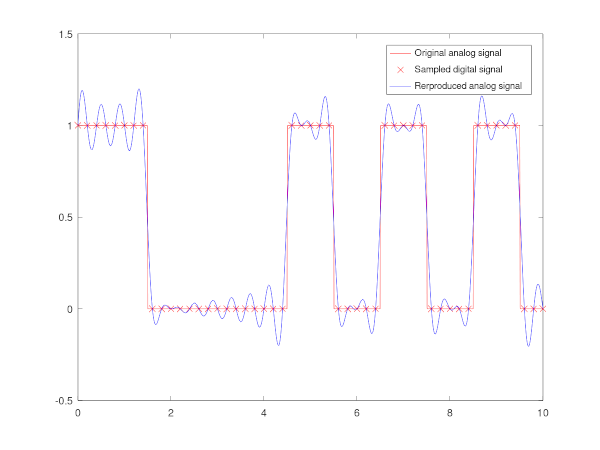
\includegraphics[width=\linewidth]{rectangletrain.png}
\end{figure}



References:
\begin{itemize}
\item 
  Tse, David., and Pramod. Viswanath. Fundamentals of Wireless Communication. Cambridge, U.K. ;: Cambridge University Press, 2005. Print.
\end{itemize}

\subsection{June---Gaussian vs. impulsive noise}


Noise is often modeled to have a \htmladdnormallink{Gaussian}{https://en.wikipedia.org/wiki/Gaussian_noise} waveform. However, it might be unrealistic in some circumstances if the \htmladdnormallink{outlier}{https://en.wikipedia.org/wiki/Outlier} events are more likely than in the Gaussian distribution. In this case, we might have to model the noise with \htmladdnormallink{fat-tailed distributions}{https://en.wikipedia.org/wiki/Fat-tailed_distribution} with significant mass in the tail distribution. 

The \htmladdnormallink{$\alpha$-stable distributions}{https://en.wikipedia.org/wiki/Stable_distribution} are used as noise models in various applications, including economics and electromagnetic communications. Also, the normal distribution belongs to the $\alpha$-stable family of $\alpha$-stable distributions ($\alpha = 2$), the only distribution in the family with a finite variance. With values $\alpha \leq 1$, the mean is undefined. The qualitative difference to the normal distribution is clear: imagine investing money in a share that has a fixed expected profit value---say, 10 euros in a year---versus investing in a share whose value fluctuates so rapidly that the expected profit (mean profit over time) can be arbitrary.

Other impulsive noise distribution models are the \textit{Middleton distributions} representing the envelope of non-Gaussian electromagnetic noise.

In the following, we compare the Gaussian and $\alpha$-stable noises. The in-phase and quadrature components are distributed as Gaussian distribution or $\alpha$-stable distribution with $\alpha =1$, accordingly. The following GNU Octave code produces plots of bandwidth-limited analog Gaussian and  $\alpha$-stable noises with $alpha = 1$. 

\begin{verbatim}
pkg load statistics

clear all;
close all;

%%Function returns the values at times T of the analog signal of the corresponding digital signal sampled at speed Fs.
function xb = digitaltoanalog(T, digitalsignal, Fs)
  xb = [];
  for t = T
    xb =  [xb sum(digitalsignal.*sinc(Fs*t - (0 : length(digitalsignal) - 1)))];
  end
end


%%Inverse of the alpha stable CDF with alpha = 1.
invalphaCDF = @(x) tan(0.5*(-1 + 2*x)*pi);
%%Generate N Alpha-stable samples.
N = 100;
alphasamples = invalphaCDF(unifrnd(0,1,1,N));

%%Generate normal samples.
normalsamples = normrnd(0,1,1,N);
%%Convert to analog signal.
T = 1 : 0.1 : N;
alphasamples = digitaltoanalog(T, alphasamples, 1);
normalsamples = digitaltoanalog(T, normalsamples, 1);

alphasamples = alphasamples/(mean(abs(alphasamples))); %Normalize by mean instantaneous amplitude.
normalsamples = normalsamples/(mean(abs(normalsamples)));
figure(1)
plot(T, alphasamples)
legend('Alpha-stable noise')
axis([0 100 -15 15])
figure(2)
plot(T, normalsamples)
legend('Gaussian noise')
axis([0 100 -15 15])


\end{verbatim}

\begin{figure}
  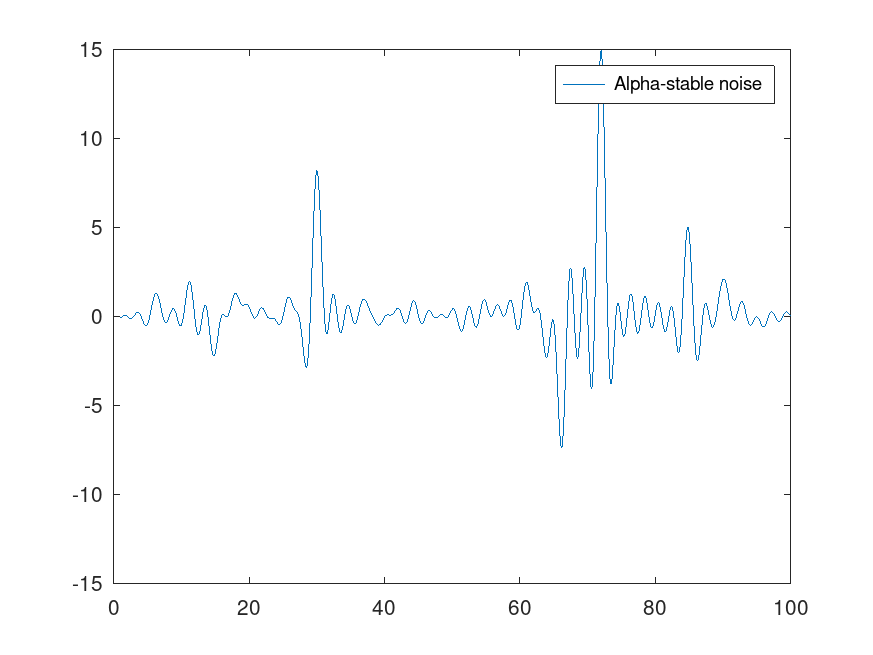
\includegraphics[width=\linewidth]{alphastablenoise.png}
\end{figure}


\begin{figure}
  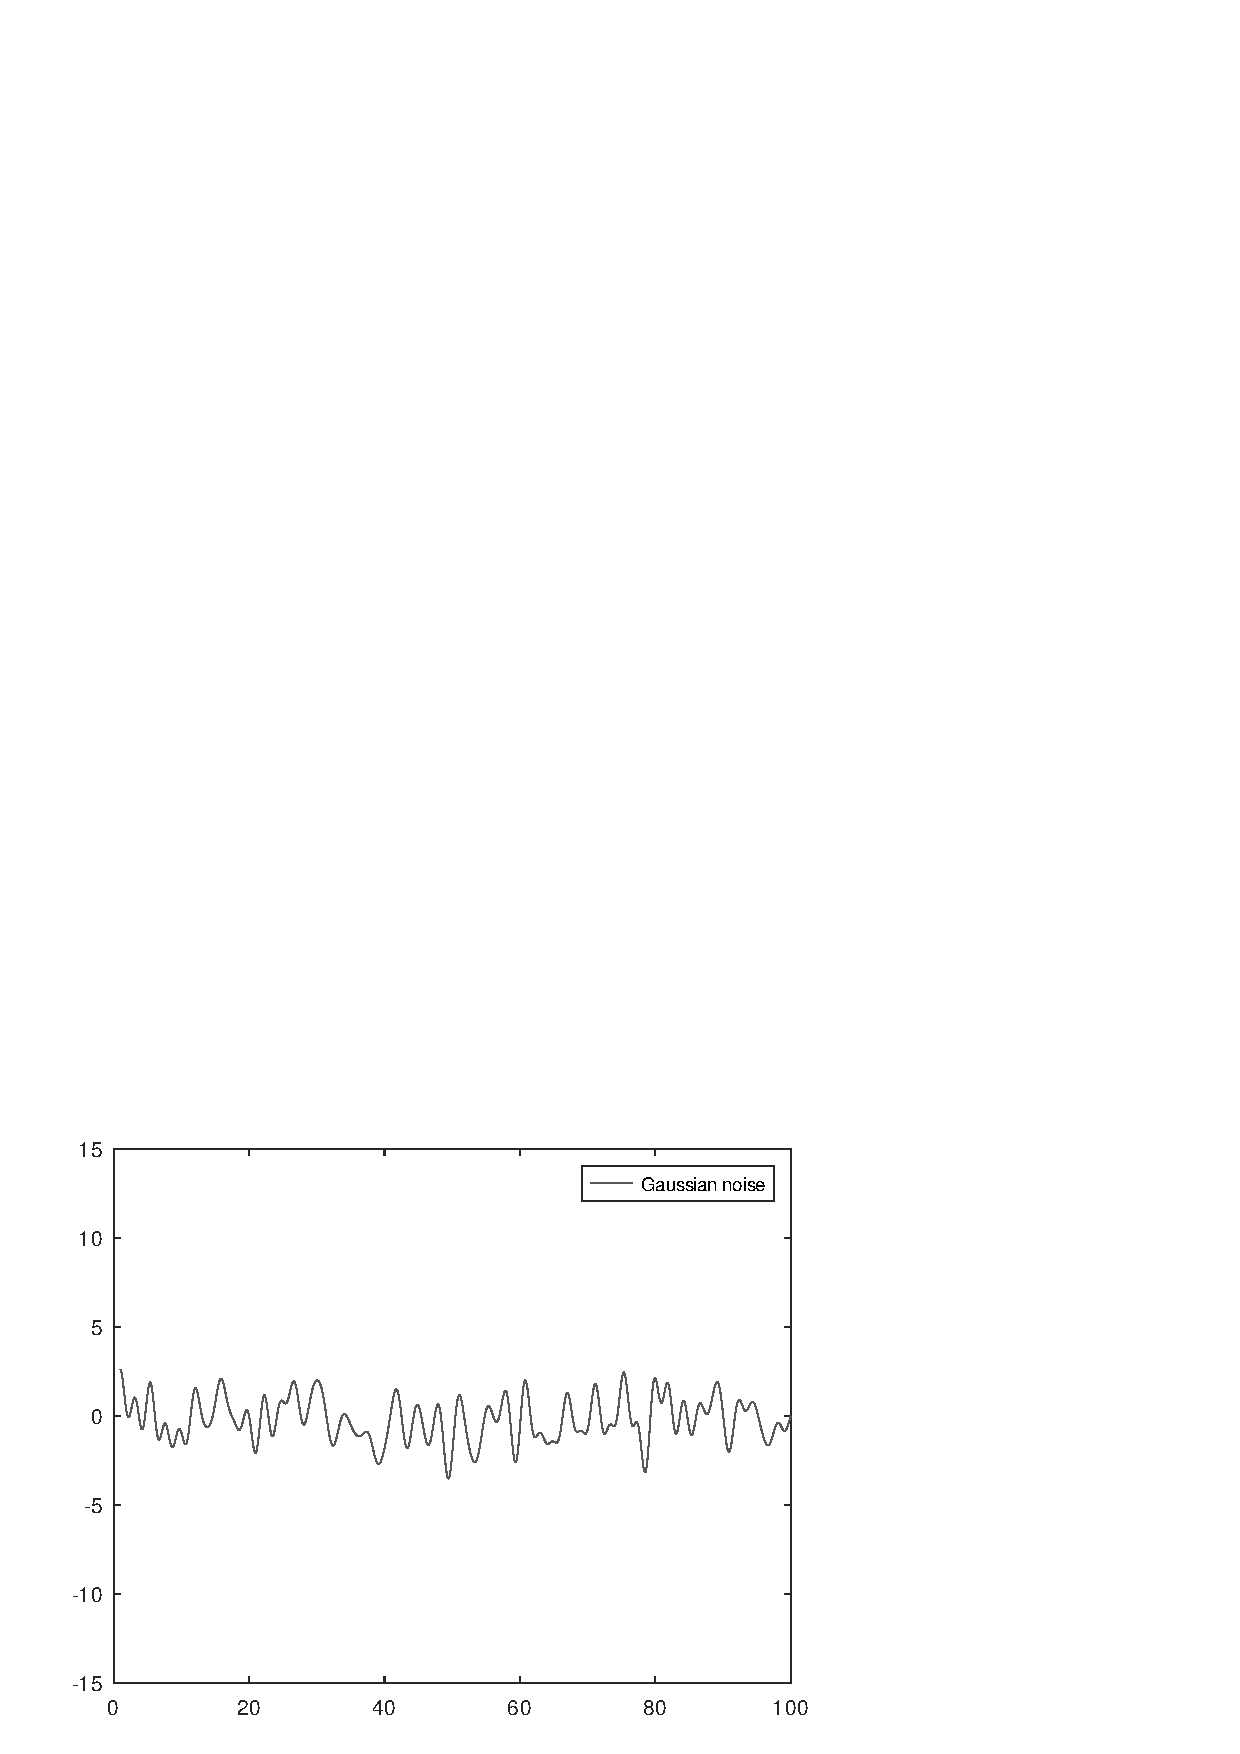
\includegraphics[width=\linewidth]{gaussiannoise.png}
\end{figure}

Comparing the figures, one can easily understand where the term ``impulsive noise'' comes from.


It is also interesting to compare the audiolized noise signals:
\htmladdnormallink{my Soundcloud}{https://soundcloud.com/ilari-angervuori/sets/gaussian-noise-and-impulsive-noise?utm_source=clipboard&utm_medium=text&utm_campaign=social_sharing}.



References:
\begin{itemize}
\item Samorodnitsky, Gennady., and Murad S. Taqqu. Stable Non-Gaussian Random Processes : Stochastic Models with Infinite Variance. New York: Chapman & Hall, 1994. Print.
\item Middleton, David. Statistical-Physical Models of Man-made and Natural Radio Noise parts I - , 1976 - .
\item 
  Tse, David., and Pramod. Viswanath. Fundamentals of Wireless Communication. Cambridge, U.K. ;: Cambridge University Press,, 2005. Print.
\end{itemize}




\subsection{July---Summing the signal powers}

Let us consider two sinusoidal signals of opposite phases during the time $t \in [0,1]$: $S_1(t) = \cos(2 \pi t)$ and $S_2(t) = \cos(2 \pi t + \pi)$. Obviously, the signals cancel each other completely, and the mean power of the additive signal $ S_1 + S_2$ is just $0$:

\begin{align}
  &\mathbb{E}[(S_1 + S_2)^2] = \int_0^1 (\cos(2 \pi t) + \cos(2 \pi t + \pi))^2dt = \int_0^10 dt = 0, \tag{1}
\end{align}
where $\mathbb{E}[\cdot]$ is the mean (slightly abusing the notation of the probabilistic expected value).


We could try to add the powers of the signals separately together:

\begin{align}
  \mathbb{E}[S_1^2] + \mathbb{E}[S_2^2] &=   \int_0^1 \cos^2(2 \pi t) dt + \int_0^1 \cos^2(2 \pi  t + \pi) dt \tag{2} \\
  &= \int_0^1 2 \cos^2(2 \pi t)  dt= \int_0^1 \cos(4 \pi t)dt + 1 = 1. \nonumber
\end{align}
But (2) significantly differs from (1)! Can we sometimes sum the individual signal powers together, which would be handy in many applications? This question has everything to do with the \htmladdnormallink{correlation}{https://en.wikipedia.org/wiki/Correlation} of the signals.

Let us assume that $S_1$ and $S_2$ are two signals. We have that
\begin{equation}
  \mathbb{E}[(S_1 + S_2)^2] = \mathbb{E}[S_1^2 + S_2^2 + 2 S_1 S_2]= \mathbb{E}[S_1^2] + \mathbb{E}[S_2^2] + 2 \mathbb{E}[S_1 S_2]. \tag{3}
\end{equation}
Hencex, the identity $\mathbb{E}[(S_1 + S_2)^2] = \mathbb{E}[S_1^2] + \mathbb{E}[S_2^2] $ holds \textit{if and only if} the \htmladdnormallink{cross-correlation}{https://en.wikipedia.org/wiki/Cross-correlation} $\mathbb{E}[S_1 S_2] = 0,$ \textit{i.e}., if the signals $S_1$ and $S_2$ are not correlated---this is not the case with our initial signals, as then the cross-correlation is given by

$$
\mathbb{E}[S_1S_2] = \int_0^1 \cos(2 \pi t) \cos(2 \pi t + \pi) dt =\int_0^1 -\cos^2(2 \pi t )dt = - \frac{1}{2}\int_0^1 \cos(4 \pi t)dt - \frac{1}{2} = - \frac{1}{2},
$$
as it should be if we tie together the equations (1), (2) and (3).

We used deterministic signals, but the same remarks apply to random signals. For example, for uniformly random phases $\phi_1,\phi_2 \in [0,2 \pi]$, let $S_1(t) = \cps(2 \pi t + \phi_1)$ and $S_2(t) = \cos(2 \pi t + \phi_2)$;

\begin{align*}
  &\mathbb{E}_{\phi_1,\phi_2} \left[\mathbb{E}[(S_1 + S_2)^2]\right] = \mathbb{E}_{\phi_1} \left[\mathbb{E}\left[ S_1^2\right]\right] + \mathbb{E}_{\phi_2} \left[\mathbb{E}\left[ S_2^2\right]\right] +\mathbb{E}_{\phi_1,\phi_2} \left[\mathbb{E}\left[ S_1S_2\right]\right] \\
  &=\frac{1}{2 \pi}\int_0^{2 \pi} \int_0^1 (\cos(2 \pi t + \phi_1))^2dt d \phi_1 + \frac{1}{2 \pi}\int_0^{2 \pi} \int_0^1 ( \cos(2 \pi t + \phi_2))^2dt  d \phi_2 \\
  &  + \frac{1}{2 \pi}\int_0^{2 \pi} \int_0^{2 \pi}\int_0^1 \cos(2 \pi t + \phi_1) \cos(2 \pi t + \phi_2)dt d \phi_1 d \phi_2\\
  &= \frac{1}{2 \pi}\int_0^{2 \pi} \int_0^1 (\cos(2 \pi t + \phi_1))^2dt d \phi_1  + \frac{1}{2 \pi}\int_0^{2 \pi} \int_0^1 ( \cos(2 \pi t + \phi_2))^2dt  d \phi_2 = 1/2 +1/2 =1.
\end{align*}
The expected powers can be summed, as the expectation of the cross-correlation $\mathbb{E}[S_1 S_2]$ is $0$ for the two random signals $S_1$ and $S_2$, \textit{i.e.}, $\mathbb{E}_{\phi_1,\phi_2} \left[\mathbb{E}\left[ S_1S_2\right]\right] =0$.


References:
\begin{itemize}
\item \htmladdnormallink{Maol-taulukot}{https://fi.wikipedia.org/wiki/MAOL-taulukot} 
\end{itemize}




%% \subsection{August – dB logplot in Mathematica}
%% In our series of Mathematica plotting, here we give an example of how to plot values in dB in a \htmladdnormallink{logarithmic plot}{https://en.wikipedia.org/wiki/Logarithmic_scale}. Among many other things, the logarithmic plot is handy in visualizing the tails of probability distributions.  We represent the values of the complementary cumulative distributions in dB, thus we have to add custom ticks for the abscissa. Also, the font size is increased and plot titles and legends are added.
%% \begin{verbatim}
%% xmax = 180;
%% ymax = 1;

%% {table1, table2, 
%%    table3} = {Table[{t, 
%%      1 - CDF[GammaDistribution[3.715287738432738`, 
%%          16.575007504627795`]][t]}, {t, 0, xmax, xmax/10}], 
%%    Table[{t, 
%%      1 - CDF[GammaDistribution[6.502676225156808`, 
%%          8.60919186301341`]][t]}, {t, 0, xmax, xmax/10}], 
%%    Table[{t, 
%%      1 - CDF[GammaDistribution[3.3444580518527207`, 
%%          16.73897127052263`]][t]}, {t, 0, xmax, xmax/10}]};

%% Labeled[Show[
%%   LogPlot[{1 - 
%%      CDF[GammaDistribution[3.715287738432738`, 16.575007504627795`]][
%%       x], 1 - CDF[
%%        GammaDistribution[6.502676225156808`, 8.60919186301341`]][x], 
%%     1 - CDF[GammaDistribution[3.3444580518527207`, 
%%         16.73897127052263`]][x]}, {x, 0, xmax}, 
%%    GridLines -> Automatic, PlotRange -> {{0, xmax}, {0, 1}}, 
%%    Ticks -> {{{0*xmax, -Infinity},
%%       {0.1*xmax, NumberForm[10*Log10[(0.1*xmax)], 3]},
%%       {0.2*xmax, NumberForm[10*Log10[(0.2*xmax)], 3]},
%%       {0.3*xmax, NumberForm[10*Log10[(0.3*xmax)], 3]},
%%       {0.4*xmax, NumberForm[10*Log10[(0.4*xmax)], 3]},
%%       {0.5*xmax, NumberForm[10*Log10[(0.5*xmax)], 3]},
%%       {0.6*xmax, NumberForm[10*Log10[(0.6*xmax)], 3]},
%%       {0.7*xmax, NumberForm[10*Log10[(0.7*xmax)], 3]},
%%       {0.8*xmax, NumberForm[10*Log10[(0.8*xmax)], 3]},
%%       {0.9*xmax, NumberForm[10*Log10[(0.9*xmax)], 3]},
%%       {1*xmax, N[NumberForm[10*Log10[(1*xmax)], 3]] "dBm"}
%%       }, {10^-4, 10^-3, 10^-2, 10^-1, 1}}, 
%%    BaseStyle -> {FontSize -> 15}, PlotStyle -> Thick], 
%%   ListLogPlot[{table1, table2, table3}, 
%%    PlotLegends -> 
%%     Placed[{"\[CapitalGamma](3.7,16.6)", "\[CapitalGamma](6.5,8.6)", 
%%       "\[CapitalGamma](3.3,16.7)"}, Right], 
%%    PlotMarkers -> {Automatic, 10}]
%%   ], {"Percent of realizations abscissa is exceeded", 
%%   "Interference power (decibel-milliwats)"}, {Left, Bottom}, 
%%  RotateLabel -> True]


%% \end{verbatim}


%% \begin{figure}
%%   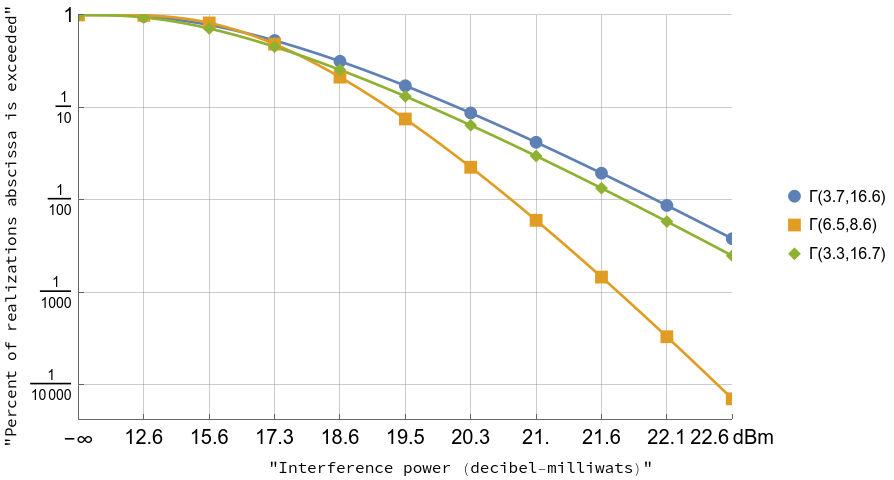
\includegraphics[width=\linewidth]{dBplot.png}
%% \end{figure}


%% References:
%% \begin{itemize}
%% \item \htmladdnormallink{reference.wolfram.com}{https://reference.wolfram.com/language/ref/LogPlot.html}
%% \end{itemize}

\subsection{September---Homography}

\htmladdnormallink{Homography}{https://en.wikipedia.org/wiki/Homography} can be used to ``change the perspective'' of an image (set of vectors). I have used homography for the satellite footprint in the computer simulations. For elevation angles smaller than $90 \degree$, you can conveniently map transmitters inside the elliptical footprint to a circle for which the radially symmetric antenna pattern function can be used. The following homography matrix $H$ transforms an \htmladdnormallink{ellipse}{https://en.wikipedia.org/wiki/Ellipse} of parameters $a$ and $b$ to a circle of radius $r$ so that the right-hand side focus point maps to the origin.
$$
H=
\begin{pmatrix}
  -a &-0 &-1 &0 &0 &0 &ar &0 &r \\
  0 &0 &0 &-a &-0 &-1 & 0& 0 &0 \\
  -c &-b^2/a& -1& 0& 0& 0 &0& 0& 0 \\
  0 &0 &0 &-c &-b^2/a &-1 &cr &rb^2/a& r\\
  a &0 &-1& 0& 0 &0 & ar &0 &-r \\
  0 &0 &0 &a &0 &-1 &0 &0 &0\\
  -c &b^2/a& -1& 0& 0& 0& 0& 0& 0 \\
  0 &0 &0 &-c &b^2/a &-1 &-rc &rb^2/ar &-r 
\end{pmatrix}
$$

\begin{figure}
  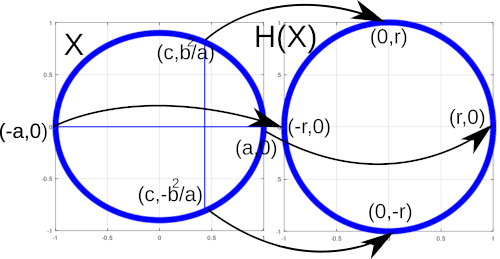
\includegraphics[width=\linewidth]{homographydrawing.png}
\end{figure}

Here is a GNU Octave code:
\begin{verbatim}

%%Changes ellipses with parameters a > b  perspective to a sphere of radius r centered in origo. Vectors to be transformed are given in 2x1000 matrix refc.

function points = homography(refc, a,b,r)
  c = sqrt(a^2 - b^2);
  %%Construct the homography matrix.
  X1 = [[-a -0 -1 0 0 0 a*r 0*r r]; [0 0 0 -a -0 -1 a*0 0*0 0]];
  X2 = [[-c -b^2/a -1 0 0 0 c*0 b^2/a*0 0]; [0 0 0 -c -b^2/a -1 c*r b^2/a*r r]];
  X3 = [[a 0 -1 0 0 0 -a*-r 0*-r -r]; [0 0 0 a -0 -1 -a*0 0*0 0]];
  X4 = [[-c b^2/a -1 0 0 0 c*0 -b^2/a*0 0]; [0 0 0 -c b^2/a -1 c*-r b^2/a*r -r]];
  P = [X1; X2; X3; X4];
  [U,S,V] = svd(P); %Singular value composition.
  h = V(:,9);
  H = reshape(h, 3, 3)';
  points = [];
  for point = refc
    homopoint = [point; 1]; %Point presented in homogeneous coordinates.
    homopoint = H*homopoint;
    homopoint = [homopoint(1)/homopoint(3); homopoint(2)/homopoint(3)];
    points = [points homopoint];
  end
  figure(1)
  plot(points(1,:), points(2,:), 'b','linewidth',10);
end

\end{verbatim}

In the following, we are rotating a ``pyramid''. It can be seen how the homography mapping can be interpreted as a change of perspective.

\begin{figure}
  \includegraphics[width=\linewidth]{gifu2.gif}
\end{figure}

References:
\begin{itemize}
\item \htmladdnormallink{Stack exchange}{https://math.stackexchange.com/questions/494238/how-to-compute-homography-matrix-h-from-corresponding-points-2d-2d-planar-homog}
\end{itemize}


\subsection{December---Asymptotic decay rate of a probability distribution}


Let us study the tail distributions of three related distributions. The asymptotic decay rate measures the thickness of a random variable's $X$ tail distribution. It is defined by
\begin{equation}
  \lim_{x \rightarrow \infty} -\frac{\log\textbf{P}(X > x)}{x}, \tag{1}
\end{equation}
where $\textbf{P}(\cdot)$ denotes the probability of an event. Let us calculate the decay rates for the exponential distribution, gamma distribution, and normal distribution.

For \textbf{exponentially distributed} $X$ with scale parameter $\theta$:
\begin{align}
  \rho_{\text{Exponential}} &=\lim_{x \rightarrow \infty} -\frac{\log\textbf{P}(X > x)}{x}  = \lim_{x \rightarrow \infty} -\frac{\log(e^{- x/\theta})}{x}   \nonumber \\
  &=\lim_{x \rightarrow \infty} -\frac{-x/\theta }{x } = 1/\theta. \tag{2}
\end{align}

For \textbf{gamma distributed} $X$ with shape parameter $k$ and scale parameter $\theta$:

\begin{align}
  \rho_{\text{Gamma}} &= \lim_{x\rightarrow \infty} -\frac{\log \mathbb{P}(X>x)}{x} = \lim_{x\rightarrow \infty} -\frac{\log (1-\gamma(k,x/\theta)/\Gamma(k))}{x} \nonumber  \\
  &=\lim_{x\rightarrow \infty} -\frac{\log (\Gamma(k,x/\theta)/\Gamma(k))}{x} \nonumber \\
  &\overset{(a)}{=} \lim_{x\rightarrow \infty} -\frac{\log (\Gamma(k,x/\theta))}{x} = \lim_{x\rightarrow \infty} -\frac{\log\left(x^{k-1}e^{-x/\theta}\right) }{x}\label{line:22} \nonumber \\
  &= \lim_{x\rightarrow \infty} -\frac{\log \left(e^{-x/\theta}\right)}{x} = 1/\theta. \tag{3}
\end{align}
In $(a)$, we used the asymptotic behavior of the gamma distribution
$$
\lim_{x \rightarrow \infty}\frac{\Gamma(s,x)}{x^{s-1}e^{-x}} = 1.
$$

For \textbf{normal distributed} $X$ with mean $\mu$ and variance $\sigma^2$:

\begin{align}
  \rho_{\text{Normal}} &= \lim_{x\rightarrow \infty} -\frac{\log \mathbb{P}(X>x)}{x} = -\lim_{x\rightarrow \infty} \frac{\log \text{erfc}\left(\frac{x-\mu}{\sigma \sqrt{2}}\right)}{x} \overset{(b)}{\geq} -\lim_{x\rightarrow \infty} \frac{\log\left( \sqrt{\frac{e}{2\pi}}e^{-2\left(\frac{x-\mu}{\sigma \sqrt{2}}\right)^2} \right)}{x} \nonumber \\
  &\geq -\lim_{x\rightarrow \infty} \frac{\log\left( e^{-2\left(\frac{x-\mu}{\sigma \sqrt{2}}\right)^2} \right)}{x} = -\lim_{x\rightarrow \infty} \frac{-2\left(\frac{x-\mu}{\sigma \sqrt{2}}\right)^2} }{x} = \frac{1}{\sigma^2 }\lim_{x\rightarrow \infty} \frac{x^2-2 x \mu + \mu^2}{ x}  = \infty, \tag{4}
\end{align}
where in $(b)$, we used the inequality $$\text{erfc}(x) \geq \sqrt{\frac{{2 e}}{\pi}} \frac{\sqrt{\beta-1}}{\beta} e^{-\beta x^2},$$ that holds for $x \geq 0$ and $\beta >1$ (we used $\beta = 2$).


The asymptotic decay rates for the exponential, gamma, and normal distribution are given in $(2)$, $(3)$, and $(4)$, respectively. We see that the decay rate $\rho$ of the normal distribution is always maximal, \textit{i.e.}, $\rho_{\text{Normal}} = \infty$. In contrast, the decay rates of the exponential and gamma distributions depend on the scale parameter $\theta$.

By normalizing the mean ($\mathbb{E}[X] = 1$) by setting $\theta = 1$ and $k=1/\theta$, we can compare the decay rates of the exponential distribution and gamma distribution: then, the decay rate of the exponential distribution is $\rho_{\text{Exponential}} = 1$ and of the gamma distribution is $\rho_{\text{Gamma}} = k$. That is, keeping the mean normalized, the gamma distribution decays slower than the exponential distribution with shape parameters $k<1$, and faster than the exponential distribution with $k>1$. With $k=1$, the distributions coincide. When $k \rightarrow \infty$, the gamma distribution approaches the normal distribution and $\rho_{\text{Gamma}} \rightarrow \rho_{\text{Normal}} = \infty$.


References:
\begin{itemize}
\item \htmladdnormallink{Error function}{https://en.wikipedia.org/wiki/Error_function}
\item \htmladdnormallink{Exponential distribution}{https://en.wikipedia.org/wiki/Exponential_distribution}
\item \htmladdnormallink{Gamma distribution}{https://en.wikipedia.org/wiki/Gamma_distribution}
\item \htmladdnormallink{Normal distribution}{https://en.wikipedia.org/wiki/Normal_distribution}

\end{itemize}

\section{Blog posts 2023}

\subsection{May---Signal fading in a satellite receiver and the coherence time}
\begin{figure}
  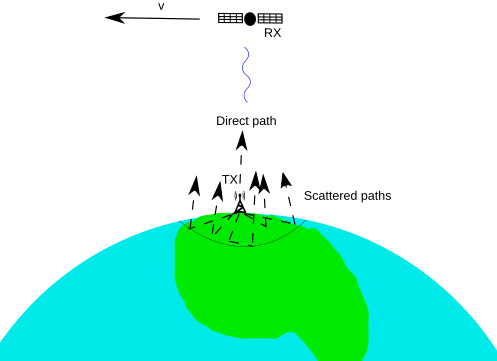
\includegraphics[width=\linewidth]{satelliteinterference.png}
\end{figure}

Let us study a faded signal in an omnidirectional satellite receiver sent by an earth transmitter. We consider that the transmitter (TX) is sending a constant \htmladdnormallink{QAM}{https://en.wikipedia.org/wiki/Quadrature_amplitude_modulation} symbol, \textit{i.e.}, the TX \htmladdnormallink{baseband signal}{https://en.wikipedia.org/wiki/Baseband} is given by
\begin{equation}
  S_{\text{TX}} = Ae^{-2 i \pi \theta}, } \tag{1}
\end{equation}
for some $\theta \in [0,1]$ and $A \in \mathbb{R}_+$. The \htmladdnormallink{passband signal}{https://en.wikipedia.org/wiki/Passband} experiences \htmladdnormallink{fading}{https://en.wikipedia.org/wiki/Fading} due to terrestrial obstacles. We use a model where $100$ scatterer objects are \htmladdnormallink{Poisson distributed }{https://en.wikipedia.org/wiki/Poisson_point_process} inside a circular area with a diameter of $180$ m. The phases of the scattered signals are independently uniformly random. Initially, the satellite, which is moving at its \htmladdnormallink{orbital speed}{https://en.wikipedia.org/wiki/Orbital_speed}, is in the \htmladdnormallink{zenith}{https://en.wikipedia.org/wiki/Zenith} w.r.t. the earth transmitter. The receiver's (RX) baseband signal is a linear combination of the \htmladdnormallink{down-conversions}{https://en.wikipedia.org/wiki/Digital_down_converter} of the scattered, \htmladdnormallink{Doppler shifted}{https://en.wikipedia.org/wiki/Doppler_effect} and \htmladdnormallink{attenuated}{https://en.wikipedia.org/wiki/Attenuation} passband signal components, and it is given by
\begin{equation}
  S_{\text{RX}}(t) = \frac{A}{l(d_0)} \sqrt{\frac{K}{K+1}}e^{-2 i \pi \tau_0(t) f_c }e^{-2 i \pi \theta} + \sum_{j=1}^{100} + \frac{A
  }{l(d_j) \sqrt{100}\sqrt{K+1}} e^{-2 i \pi \tau_j(t) f_c }e^{-2 i \pi \theta}, \tag{2}
\end{equation}
where $l(d_i)$ is the path-loss function at distance $d_j$ from the scatterer $j$, $d_0$ is the direct-path distance to the transmitter, $K$ is the parameter that determines the energy ratio of the direct-path (\htmladdnormallink{LOS}{https://en.wikipedia.org/wiki/Line-of-sight_propagation}) component and the scattered paths, and $\tau_j(t) = d_j(t)/c$ is the propagation delays restricted by the speed of light $c$, which is dependent on time $t$ as the satellite moves, and $f_c$ is the carrier frequency.

Given this model, we are interested in the time scale during which $S_{\text{RX}}(\cdot)$ varies, \textit{i.e.}, the \htmladdnormallink{coherence time}{https://en.wikipedia.org/wiki/Coherence_time_(communications_systems)}. The coherence time depends on the Doppler shift, and the satellite's orbital speed is given by
\begin{equation}
  v = \sqrt{\frac{GM}{h + R_{\oplus}}}, \tag{3}
\end{equation}
where $GM \approx 3.9 \cdot 10^{14}$m$^3/$s$^2$, and the denominator is the sum of the satellite's altitude and the earth's radius, respectively. This is fast: around $7$ km/s at $h=600$ km. However, Doppler shift is only caused by the velocity component that is directed towards the transmitter. The Doppler shift is zero when the satellite is in the zenith and grows at lower \htmladdnormallink{elevation angles}{https://en.wikipedia.org/wiki/Horizontal_coordinate_system}. In our model, the scatterers were distributed in an area of diameter $180$ m below the satellite, and the maximum Doppler shift initially is $50$ Hz for $f_c = 12 \cdot 10^{9}$; hence, the Doppler spread is $D_s = 100$ Hz. A small estimate for the coherence time is given by
\begin{equation}
T_c = \frac{1}{8 D_s} \approx  10^{-3} \text{s}. \tag{4}
\end{equation}
The satellite moves about $8$ meters during this period.

The following figures illustrate the RX baseband signal changing in time while the satellite moves. As expected, the variance in the signal strength is larger in the Rayleigh faded case.

\begin{figure}
  \includegraphics[width=\linewidth]{basebandgifK10.gif}
  \caption{The baseband signal with partial LOS $K=10$.}
\end{figure}

\begin{figure}
  \includegraphics[width=\linewidth]{basebandgifK0.gif}
  \caption{The baseband signal under Rayleigh fading $K=0$.}
\end{figure}

Here is the Octave code:

\begin{verbatim}
function signals = satellite_baseband_simulation()
  pkg load statistics
  close all;
  clear all;
  clear imread;
  clear imwrite;

  h = 600*1000; #Altitude of satellites.
  K = 0; #Rician parameter.
  t = 0; #Initial time.
  [refs bbsignals] = scatteredsignals(K);  #Random baseband signals ''bbsignals' and the scatterer-obstacle's locations in 'refs'.
  signal = RXbaseband(refs, bbsignals);
  N = 200;
  history =[];
  filename = 'basebandgif.gif';
  if(exist(filename))
    delete(filename);
  end


  for iii = 1 : N
    ##Observe the progress.
    if(mod(iii,10) == 0)
      iii
    end
    refs = rotateearth(refs); #Rotate Earth.
    signal = RXbaseband(refs, bbsignals); #New received baseband signal
    history = [history [real(signal); imag(signal)]]; #History of the signals.    
    ##Write GIF.
    quiver(0,0,real(signal), imag(signal));
    hold on;
    plot(history(1,:), history(2,:))
    axis([[-0.1, 0.1], [-0.1, 0.1]]);
    t = t + 1/(4*8*100); #Time hop. t = 1/(8*300) is the initial coherence time of the example.
     text(0.03, 0.03, mat2str(t, 3), 'fontsize',25);
    text(0.075, 0.03, 's', 'fontsize',25);
    frame = getframe();
    imwrite(frame.cdata, filename,'gif','writemode','append','DelayTime',0.05, 'Compression','lzw')
    hold off;
  end  
end


##Returns a table of 101 (1 LOS signal and 100 signals from the scattered paths) randomly phased complex baseband signal symbols each corresponding to one of a obstacle location given in 'refs'. 'K' is the Rician parameter.
function [refs, signals] = scatteredsignals(K)
  ##First, generate the Poisson distributed random obstacle locations.
  refs = [0; 0]; #LOS component.
  yMin = 1-0.0000000001; yMax = 1;
  xMin = -pi; xMax = pi;
  xDelta = xMax - xMin; yDelta = yMax - yMin; #Rectangle dimensions
  numbPoints =100;    #Number of points.
  x = xDelta*(rand(numbPoints,1)) + xMin;    #Pick points from uniform distribution
  y = yDelta*(rand(numbPoints,1)) + yMin;    
  refs = [refs [pi/2-asin(y)' ; x'] ]; #Map referencepoints to spherical coordinates
  A = 30000; #Amplitude.
  signals = [A*sqrt(K/(K+1)).*exp(-rand(1,1).*i*2*pi)];
  signals = [signals A/(sqrt(100)*sqrt(1+K)).*exp(-rand(1,length(refs(1,:))-1).*i*2*pi)];
end


##Derives the received baseband signal.
function bb = RXbaseband(refs, signals)
  R = 6378*1000; #Radius of Earth in m.
  h = 600*1000; #Altitude of the satellite.
  d = @(gamma) sqrt((cos(gamma).*(R+h)-R).^2+(sin(gamma).*(R+h)).^2); ##Distance to the satellites in m.
  c = 299792458; ##Speed of light.
  if(!isempty(refs))
    a = 1./d(refs(1,:));
    tau  = d(refs(1,:))/c;
  else
    a = 0;
    tau = 0;
  end
  fc = 12*10^9; ##Modulation frequency.
  ab = a.*exp(-i*2*pi*tau.*fc); ##Received individual signals.
  bb = sum(ab.*signals); ##Aggregate received signal.
end

##Rotates the positions in 'refs' as the satellite "moves". In this model, the satellite stays still at (0,0) but the Earth moves.
function refs = rotateearth(refs)
  t = 1/(4*8*100); #Time hop in seconds.
  h= 600*1000; #Altitude of the satellite.
  R = 6378*1000; #Radius of Earth.
  GM = 3.986*10^14; #Gravitational constant.
  orbitalspeed = sqrt(GM/(h + R)); #Satellite speed in m/s.
  angularspeed = orbitalspeed/(h + R); #Angular speed of the satellite.
  rotation = angularspeed*t; #Rotation of Earth.
  eucpos  = pol2euc(refs); #Transform the polar coordinates to euclidean coordinates.
  newpos = [[1 0 0]; [0 cos(rotation) -sin(rotation)]; [0 sin(rotation) cos(rotation)]]*eucpos; #Rotation about x-axis.  
  refs = euc2pol(newpos); #Back to the polaroordinates.
end


function p  = euc2pol(e)
  R = 6378*1000; #Radius of Earth.
  p = [acos(e(3,:)./R); (e(2,:) >= 0).*atan2(e(2,:),e(1,:)) + ...
			(e(2,:) < 0).*(atan2(e(2,:),e(1,:)) + 2*pi)]; #Polar coordinates from the given Euclidean coordinates in 'e'..
end

function e = pol2euc(p)
  R= 6378*1000; #Radius of Earth.
  e = [R*cos(p(2,:)).*sin(p(1,:));...
       R*sin(p(2,:)).*sin(p(1,:));...
       R*cos(p(1,:))]; #Euclidean coordinates from the given polar coordinates in 'p'.
end

\end{verbatim}
References:
\begin{itemize}
\item Tse, David., and Pramod. Viswanath. Fundamentals of Wireless Communication. Cambridge, U.K. ;: Cambridge University Press,, 2005.


\section{Blog posts 2024}

\subsection{March---A representation of the generalized hypergeometric function $_3F_2$}


Here is a representation of the \htmladdnormallink{hypergeometric function}{https://en.wikipedia.org/wiki/Generalized_hypergeometric_function} $_3F_2(1,1,b;2,2;\cdot)$ in terms of the \htmladdnormallink{polylogarithm}{https://en.wikipedia.org/wiki/Polylogarithm}: For  $|x|<1$ and $b\in\mathbb{N}$, the \textit{hypergeometric series} representation is given by
                 \begin{align*}
                   &  _3F_2(1,1,1+b;2,2;x)= \sum^{\infty}_{n=0}\frac{(1)_n(1)_n(1+b)_n}{(2)_n(2)_n} \frac{x^n}{n!} \nonumber\\
                   &=\sum^{\infty}_{n=0}\frac{(1+b)_n}{(n+1)^2n!}x^n = \frac{1}{b!}\sum^{\infty}_{n=0} \frac{(n+1)_{b}}{(n+1)^2}x^n \nonumber \\
                   &\overset{(a)}{=} \frac{1}{b!} \sum^{\infty}_{n=0} \frac{\sum^{b}_{k=1}\left[ b \atop k \right](n+1)^k}{(n+1)^2} x^n\nonumber \\
                   &= \frac{1}{b!} \sum^{b}_{k=1}\left[ b \atop k \right] \sum^{\infty}_{n=0}  \frac{x^n}{(n+1)^{2-k}} \overset{(b)}{=} \frac{1}{b!}\sum^{b}_{k=1} \left[ b \atop k \right]\frac{\text{Li}_{2-k}(x)}{x}, \label{eq:pollog}
                 \end{align*}
                 where $\left[ b \atop k \right]$ is the unsigned Stirling number of the first kind. In (a), we used the expansion of the rising Pochhammer factorial and in (b), we used the definition of the polylogarithm. Furthermore, the $x \in \mathbb{C}$ follows from the \htmladdnormallink{analytic continuation}{https://en.wikipedia.org/wiki/Analytic_continuation} of the polylogarithm.


\end{document}



%
% optional post-title formatting for PostScript
%
\parindent0pt
\parskip2.5ex plus 0.5ex minus 0.5ex



